%%
%% This is file `proposal.tex',
%% generated with the docstrip utility.
%%
%% The original source files were:
%%
%% samples.dtx  (with options: `all,journal,bibtex,acmsmall')
%% 
%% IMPORTANT NOTICE:
%% 
%% For the copyright see the source file.
%% 
%% Any modified versions of this file must be renamed
%% with new filenames distinct from proposal.tex.
%% 
%% For distribution of the original source see the terms
%% for copying and modification in the file samples.dtx.
%% 
%% This generated file may be distributed as long as the
%% original source files, as listed above, are part of the
%% same distribution. (The sources need not necessarily be
%% in the same archive or directory.)
%%
%%
%% Commands for TeXCount
%TC:macro \cite [option:text,text]
%TC:macro \citep [option:text,text]
%TC:macro \citet [option:text,text]
%TC:envir table 0 1
%TC:envir table* 0 1
%TC:envir tabular [ignore] word
%TC:envir displaymath 0 word
%TC:envir math 0 word
%TC:envir comment 0 0
%%
%% The first command in your LaTeX source must be the \documentclass
%% command.
%%
%% For submission and review of your manuscript please change the
%% command to \documentclass[manuscript, screen, review]{acmart}.
%%
%% When submitting camera ready or to TAPS, please change the command
%% to \documentclass[sigconf]{acmart} or whichever template is required
%% for your publication.
%%
%%
\documentclass[acmsmall, nonacm]{acmart}
%%
%% \BibTeX command to typeset BibTeX logo in the docs
\AtBeginDocument{%
  \providecommand\BibTeX{{%
    Bib\TeX}}}

%% Rights management information.  This information is sent to you
%% when you complete the rights form.  These commands have SAMPLE
%% values in them; it is your responsibility as an author to replace
%% the commands and values with those provided to you when you
%% complete the rights form.


%%
%% Submission ID.
%% Use this when submitting an article to a sponsored event. You'll
%% receive a unique submission ID from the organizers
%% of the event, and this ID should be used as the parameter to this command.
%%\acmSubmissionID{123-A56-BU3}

%%
%% For managing citations, it is recommended to use bibliography
%% files in BibTeX format.
%%
%% You can then either use BibTeX with the ACM-Reference-Format style,
%% or BibLaTeX with the acmnumeric or acmauthoryear sytles, that include
%% support for advanced citation of software artefact from the
%% biblatex-software package, also separately available on CTAN.
%%
%% Look at the sample-*-biblatex.tex files for templates showcasing
%% the biblatex styles.
%%

%%
%% The majority of ACM publications use numbered citations and
%% references.  The command \citestyle{authoryear} switches to the
%% "author year" style.
%%
%% If you are preparing content for an event
%% sponsored by ACM SIGGRAPH, you must use the "author year" style of
%% citations and references.
%% Uncommenting
%% the next command will enable that style.
%%\citestyle{acmauthoryear}


%%
%% end of the preamble, start of the body of the document source.
\begin{document}

%%
%% The "title" command has an optional parameter,
%% allowing the author to define a "short title" to be used in page headers.
\title[CSDS490 Project Final Report]{Deep Neural Network-based Dual Watermarking for Image Security}

%%
%% The "author" command and its associated commands are used to define
%% the authors and their affiliations.
%% Of note is the shared affiliation of the first two authors, and the
%% "authornote" and "authornotemark" commands
%% used to denote shared contribution to the research.
\author{Chentao Fan}
\authornote{Both authors contributed equally to this project.}
\email{cxf373@case.edu}
\affiliation{%
  \institution{cxf373, Case Western Reserve University}
  \city{Cleveland}
  \state{Ohio}
  \country{USA}
}

\author{Yihao Zhang}
\authornotemark[1]
\email{yxz3114@case.edu}
\affiliation{%
  \institution{yxz3114, Case Western Reserve University}
  \city{Cleveland}
  \state{Ohio}
  \country{USA}
}

%%
%% By default, the full list of authors will be used in the page
%% headers. Often, this list is too long, and will overlap
%% other information printed in the page headers. This command allows
%% the author to define a more concise list
%% of authors' names for this purpose.
% \renewcommand{\shortauthors}{Chentao & Author}

%%
%% The abstract is a short summary of the work to be presented in the
%% article.
\begin{abstract}
  A final report for CSDS490 final project.
\end{abstract}


%%
%% Keywords. The author(s) should pick words that accurately describe
%% the work being presented. Separate the keywords with commas.
\keywords{Python, Machine Learning}


%%
%% This command processes the author and affiliation and title
%% information and builds the first part of the formatted document.
\maketitle


\section{Project Overview}\label{sec:project-overview}

% Give a summary review of your project, highlighting its purpose and goals

% Briefly review the expected impact or benefits of the project as set out at the start, and how the end result meets those expectations or set new ones.

\subsection{Overview}\label{subsec:overview}
The project aims to reconstruct a deep learning-based dual watermarking
technique for image copyright protection and authentication.
The technique will embed two types of watermarks into digital images: a
perceptual hash for copyright protection and a cryptographic hash for
content and source authentication.
And we will also implement an Android application to show how to use our model into a real-world application.

\subsection{Background}\label{subsec:background}

The rapid advancement of digital technology in the domain
of image processing has paved the way for creating
high-resolution digital content.
Side-by-side, this advanced
technology also helps the attacker to launch attacks on digital
content, such as illegally manipulating, duplicating, or accessing
information without the owners’ knowledge, violating
the integrity, authenticity, and copyright protection of the
target digital content.
Therefore, developing secure copyright protection and authentication has become a challenging task.

Digital watermarking is an effective technique for achieving
copyright protection and authentication.
The process of digital
watermarking involves two primary operations: watermark
embedding and watermark extraction.

In general, there are two types of digital watermarks addressed
in the existing literature: visible and invisible watermarks.
A visible watermark typically contains a visible
message or a logo as a watermark in digital content.
On the other hand, in invisible watermarking, a watermark is embedded
and remains invisible, such that the digital media appears
visually similar to the original image.

Invisible watermarks can be broadly classified into fragile and robust watermarks.
Fragile watermarking is used in applications where even a
single-bit change in the content is not allowed, as the single-bit change in the digital content will alter
the watermark and will make it invalid.
Therefore, fragile watermarking is used in digital content authentication and
integrity verification.
Robust watermarking shows robustness
against content-preserving image manipulations, such as resizing,
rotation, flipping, format conversion, etc, which makes it the most suitable watermarking technique
for copyright protection.
However, the degree of robustness is application-specific.

The most prominent technique for calculating the perceptual
hash is the Discrete Cosine Transformation (DCT) technique. In this technique, the input image is
expressed in terms of cosine functions oscillating at different
frequencies. Frequency coefficients representing the lower
frequency components contain important features of an image
that are robust against distortions.

\begin{figure}[ht]
  \centering
  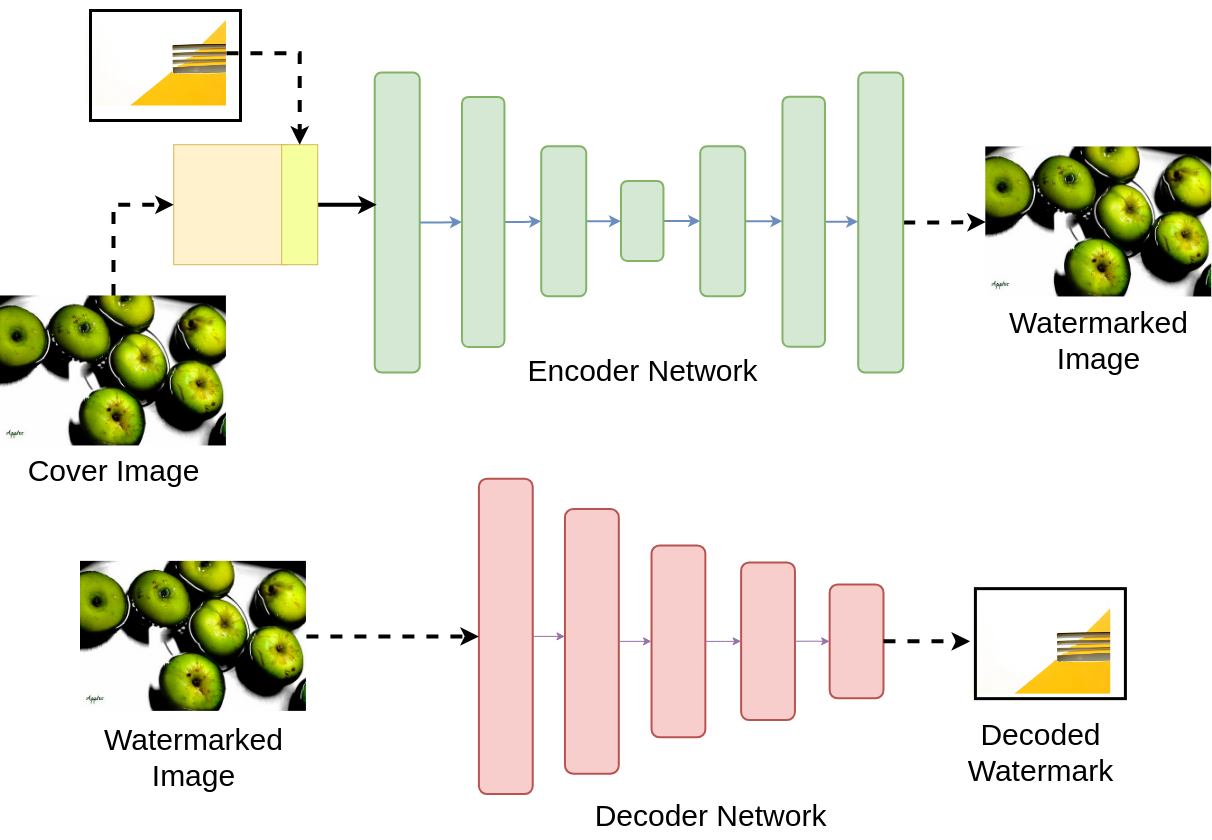
\includegraphics[width=0.5\textwidth]{imgs/nn2.png}
  \caption{General overview of deep learning-based watermarking where an encoder network is used for embedding the watermark and the decoder network is used for extracting the watermark.} %centre caption above image
  \label{fig:encoder-decoder}
  \Description{General overview of deep learning-based watermarking where an encoder network is used for embedding the watermark and the decoder network is used for extracting the watermark.}
\end{figure}

\section{Problem Statement}\label{sec:problem-statement}

% • Briefly review the problem or challenge that your project originally aimed to address

% • Discuss any existing solutions or approaches to the problem and their limitations

\subsection{Problem}\label{subsec:problem}

Deep learning-based watermarking techniques are the newest approach that can efficiently watermark images by overcoming the drawbacks of traditional watermarking techniques~\cite{ref4,deepwatermark1,fang2020deep,li2021survey}. In deep learning-based watermarking, encoder and decoder networks are used to perform watermarking, as shown in \autoref{fig:encoder-decoder}. The encoder network constructs a watermarked image by embedding the watermark into the cover image, as shown in the upper part of \autoref{fig:encoder-decoder}.  Once the watermarked image is constructed, the decoder network (shown at the bottom part of \autoref{fig:encoder-decoder}) is used to extract the watermark from the watermarked image.

Deep learning-based watermarking has its own challenges. The fragile nature of $DNN$ can sometimes cause the model to fail~\cite{lacuna2}. As a result, fully utilizing the ability of deep neural networks to learn automatically and generalizing it to both watermark embedding and extracting processes is difficult. The lack of a good balance of imperceptibility and robustness is also a major concern in deep learning-based watermarking~\cite{lacuna1,lacuna6,deepwatermark1,lacuna4,lacuna5}.

\subsection{Example}\label{subsec:example}

Traditional image watermarking methods like DCT are not robust against
content-preserving image manipulations and lack inherent watermark
verification. Deep learning-based watermarking techniques, while more
robust, still face challenges in maintaining a balance between
robustness and imperceptibility and are vulnerable to overwriting and
surrogate model attacks.

Relevant examples to emphasize the problem:

\begin{itemize}
  \item Rotation or blurring of an image can distort embedded watermarks in
        traditional methods.
  \item Overwriting attacks can replace the original
        watermark with an attacker's watermark, compromising copyright
        protection.
\end{itemize}

\subsection{Solution}\label{subsec:solution}

Existing solutions include traditional watermarking techniques and
single watermarking deep learning methods. However, these solutions are
limited in their robustness and adaptability, and they do not address
the need for source authentication and protection against overwriting
attacks.

We propose a deep learning-based invisible dual watermarking technique that has all the features mentioned above.  This dual watermarking technique serves two objectives at once:

\begin{itemize}
  \item Protecting digital content copyright
  \item Content and Source authentication
\end{itemize}

Perceptual hash is used as the first watermark for protecting digital content copyright, whereas cryptographic hash is used as the second watermark for content and source authentication.

\section{Methodology}\label{sec:methodology}

% • Outline the approach or methodology you planned to follow in order to accomplish the project objectives.

% • Pay particular attention to areas of the project that were not fully decided on or known only at a high level in the proposal and/or interim report.
\subsection{Hashing}\label{subsec:hashing}

Hashing is a well-known concept in the domain of cryptography~\cite{lin1998generating}, through which a unique digest of a given message is generated. Cryptographic hash functions are generally used in digital signatures, message authentication codes, and to check the integrity of a message, image, or digital file~\cite{crypto}.

\subsubsection{Cryptographic Hash}\label{subsubsec:cryptographic-hash}

Secure Hash Algorithm ($SHA$) is one of the standard cryptographic hash functions with a strong avalanche effect, which means any tiny change to the input will lead to a significant change at the output (hash value)~\cite{chen2022asymmetric,crypto,lin1998generating}. When it comes to image processing, cryptographic hash becomes less useful, specifically where certain perceptual content-preserving image manipulations, such as JPEG compression, noise, blurring, cropping, deformations, etc, are allowed as these manipulations will alter the hash value.

\subsubsection{Perceptual Hash}\label{subsubsec:perceptual-hash}

In this line, the perceptual hash is a class of comparable hash functions that generate a distinct and unique hash using robust or invariant features present in the input image~\cite{phash2, thesis,phash1,phashcopy2,ref8,qamra2005enhanced} such that two visually similar images should produce the same perceptual hash value. There are four basic techniques for generating perceptual hash: frequency transformations, dimensionality reduction, statistical methods,  and extracting the local features of an image~\cite{ref10}.

The most prominent technique for calculating the perceptual hash is the Discrete Cosine Transformation ($DCT$) technique~\cite{phash-dct,phash-dct1,phash-dct3}.

\begin{figure}[ht]
  \centering
  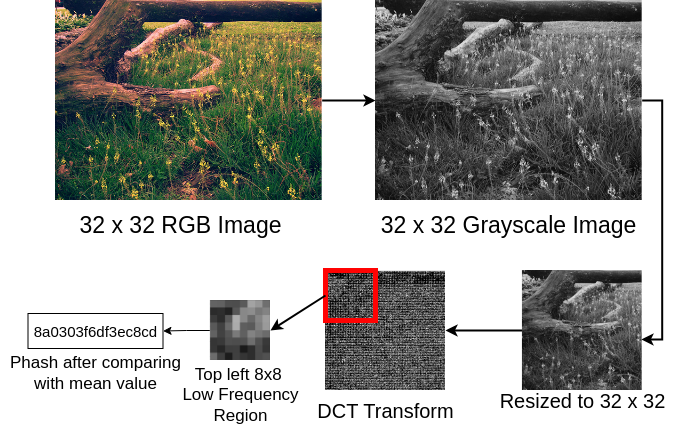
\includegraphics[width=0.5\textwidth]{imgs/phash.png}
  \caption{Perceptual hash generation process} %centre caption above image
  \label{fig:phash}
  \Description{The perceptual hash generation process. The input image is resized to $32 \times 32$ pixels, and then the $DCT$ transformation is applied to convert the image into the frequency domain. The perceptual hash is generated by comparing the frequency coefficients in the low-frequency block with the mean value of all the coefficients in that block.}
\end{figure}

As shown in \autoref{fig:phash}, in this technique, the input image is expressed in terms of cosine functions oscillating at different frequencies. Frequency coefficients representing the lower frequency components contain important features of an image that are robust against distortions. In $ DCT$-based perceptual hash, the input color image is first converted into a grayscale image and resized to $32 \times 32$ pixels. The grayscale image is then converted to the $32 \times 32$ frequency domain image through $DCT$ transformation. The   $8 \times 8$ block of pixels in the upper-left portion of the image represents the low-frequency block of the resized grayscale image. Each frequency coefficient present in the low-frequency block of pixels is compared to the mean value of all the frequency coefficients of pixels in the low-frequency block.  If the value of an individual frequency coefficient is greater than the mean value, its phase is taken as $1$, and if it is not, it is taken as $0$. The final hash is obtained by arranging the 64-bit binary values sequentially, thus representing the perceptual hash of an image.

\begin{table}[hb]
  \centering
  \begin{tabular}{|c|c|c|c|c|}
    \hline
    \textbf{Modification} & \textbf{SHA3 Hash}    & \textbf{Perceptual Hash} & \textbf{Similarity} & \textbf{Image}                                                 \\
    \hline
    Original Image        & 3970ad8d98939ec3\dots & 91d3eaed4662d904         & 100\%               & \includegraphics[width=0.1\textwidth]{test phash/im1.jpg}      \\
    \hline
    Dot Modified Image    & cbfb16ece37b3371\dots & 91d3eaed4662d904         & 100\%               & \includegraphics[width=0.1\textwidth]{test phash/im1_dot.jpg}  \\
    \hline
    Blurred Image         & f569535b93f1243b\dots & 91d3eaed4662d904         & 100\%               & \includegraphics[width=0.1\textwidth]{test phash/im1_blur.jpg} \\
    \hline
    Cropped Image         & af448d68d5be9839\dots & 99b5768aa1b172ca         & 76\%                & \includegraphics[width=0.1\textwidth]{test phash/im1_crop.jpg} \\
    \hline
    Text Modified Image   & 4120d048987860d2\dots & 91d3eaed4662d904         & 100\%               & \includegraphics[width=0.1\textwidth]{test phash/im1_text.jpg} \\
    \hline
  \end{tabular}
  \caption{Example of perceptual hash values and SHA3 hash values for different images.}
  \label{tab:perceptual-hash-example}
\end{table}

\begin{figure}[hb]
  \centering
  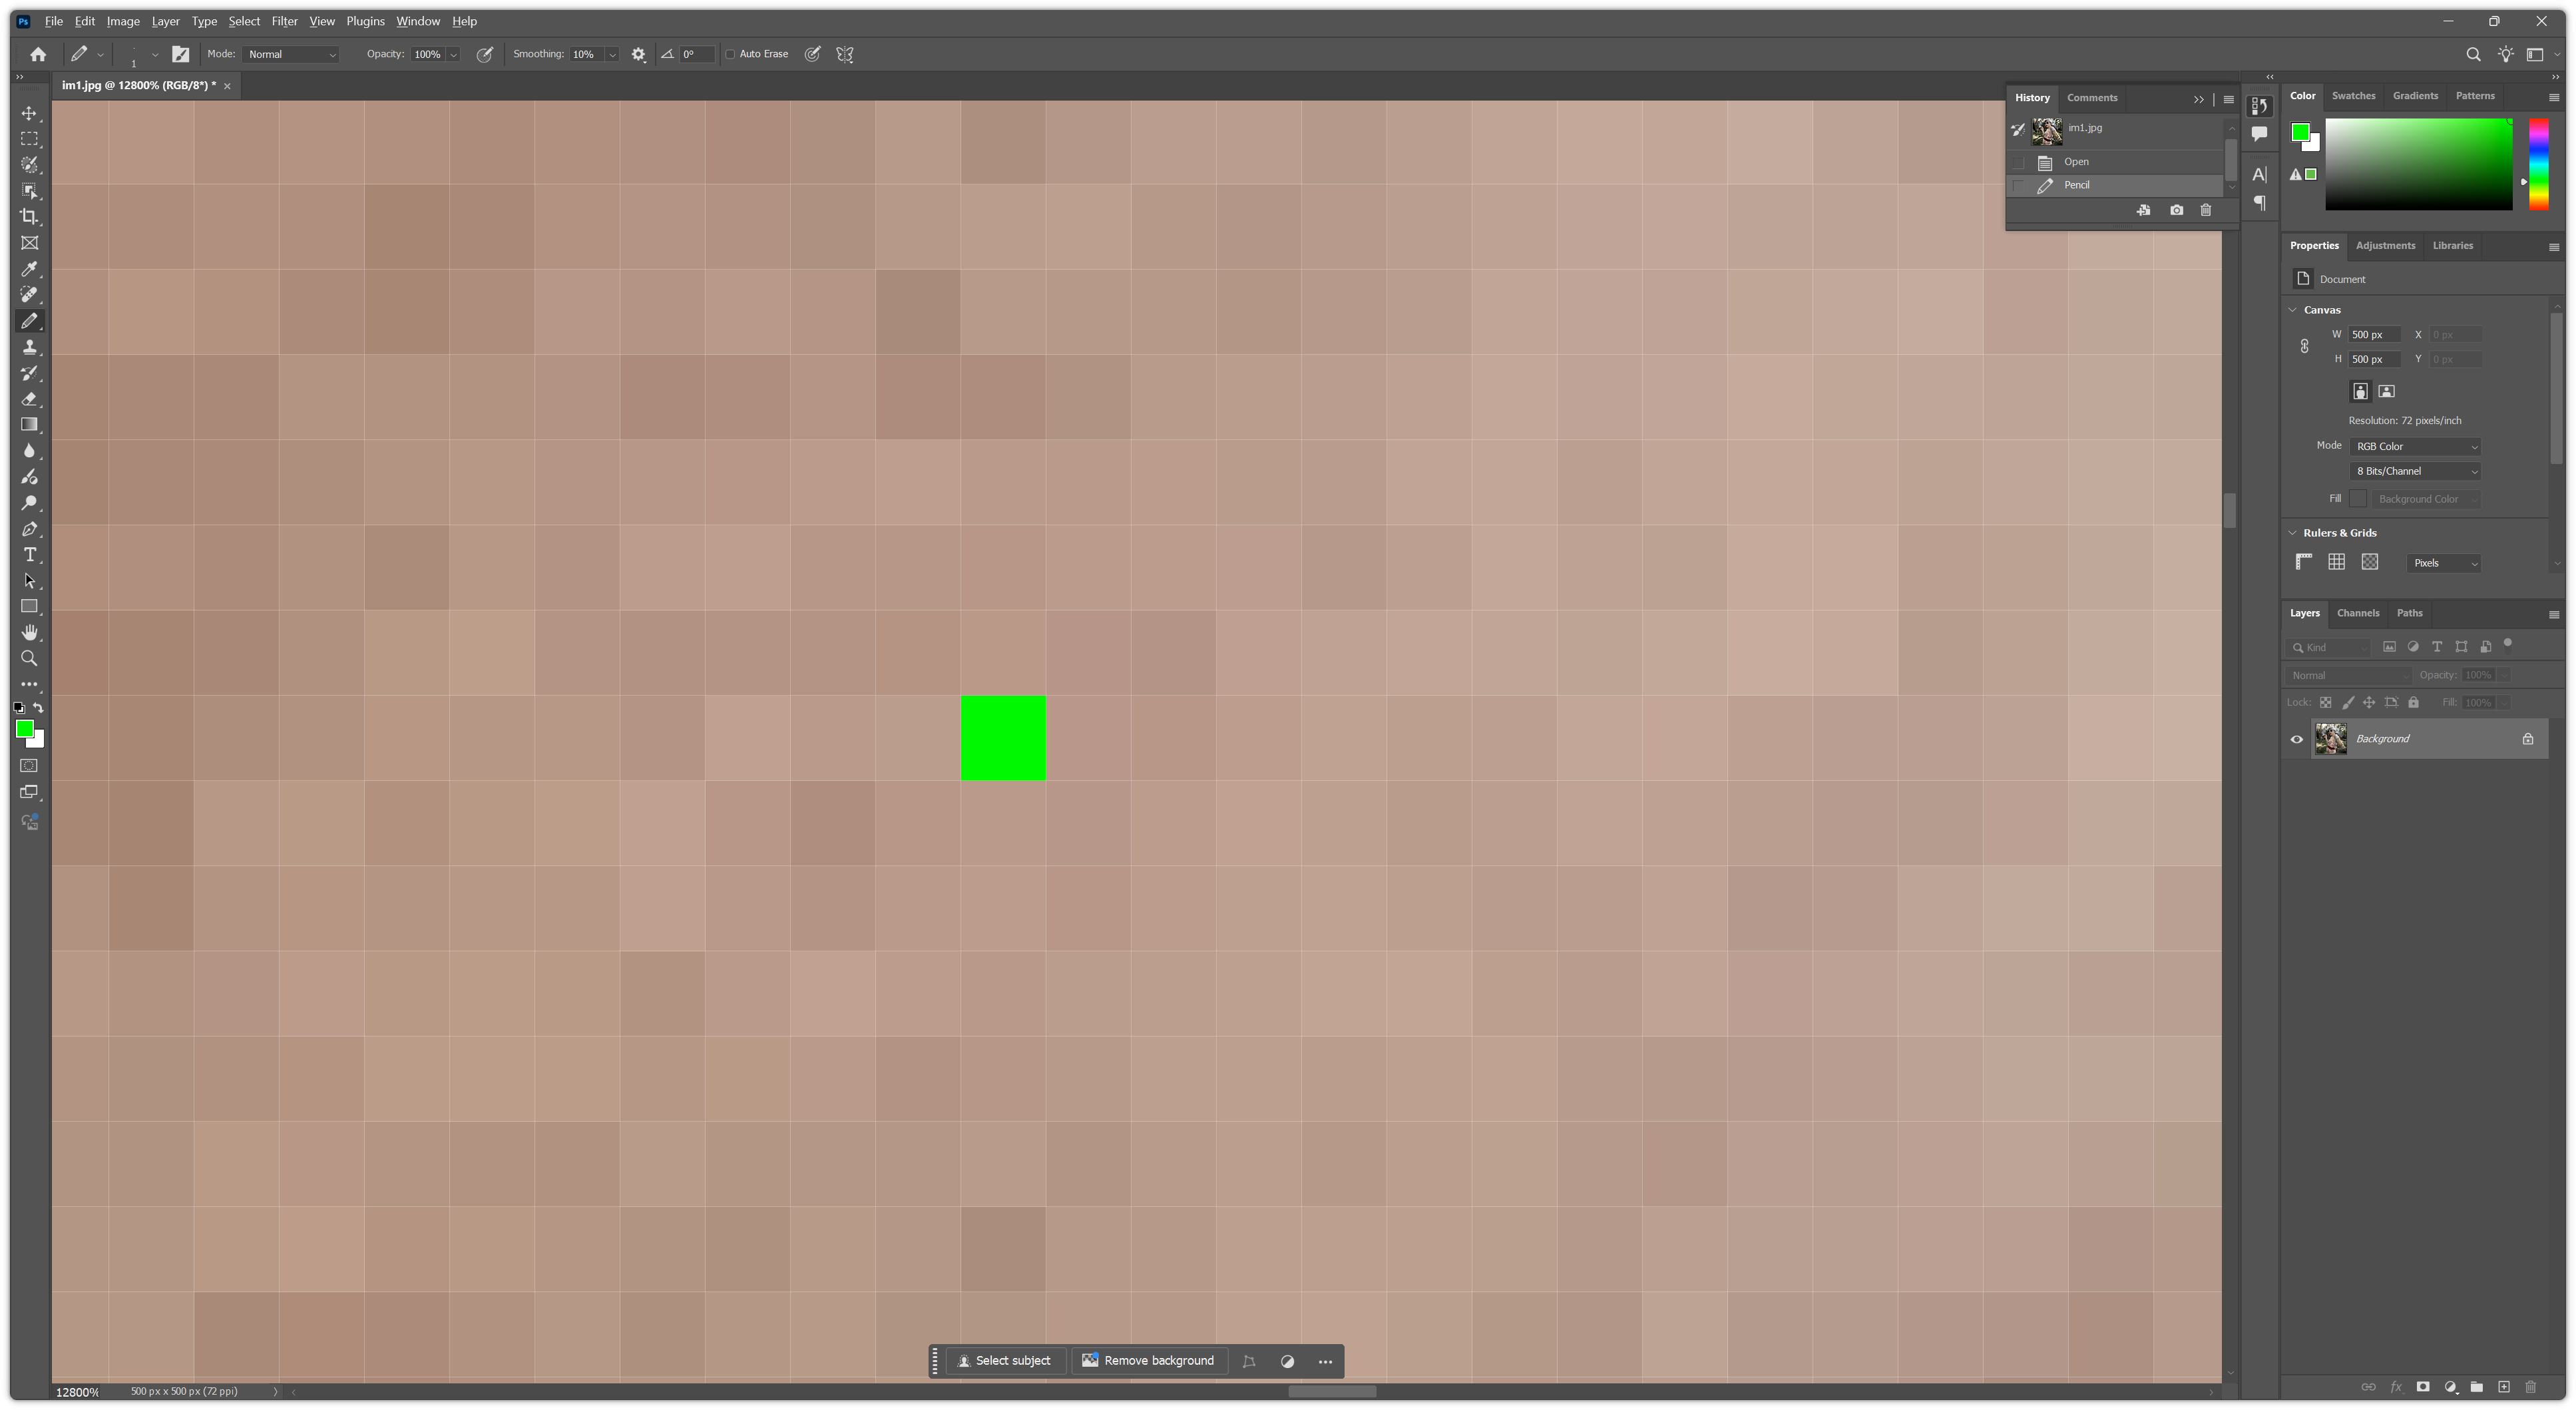
\includegraphics[width=\textwidth]{imgs/dot-modified-image.png}
  \caption{Photoshop screenshot for dot modification} %centre caption above image
  \label{fig:dot-modified-image}
  \Description{Photoshop screenshot for dot modification. The original image is modified by adding a dot in the center of the image.}
\end{figure}

\subsubsection{Example}\label{subsubsec:example}

The obtained perceptual hash will not vary if the image remains perceptually the same while SHA3 hash would not. As \autoref{tab:perceptual-hash-example} shows, the perceptual hash value of the original image and the modified image is the same, while the SHA3 hash value is different.





For the dot modified image, the dot is modified using Photoshop as shown in \autoref{fig:dot-modified-image}.

\subsection{Watermark Embedding} \label{subsec:watermark-embedding}

\begin{figure}[ht]
  \centering
  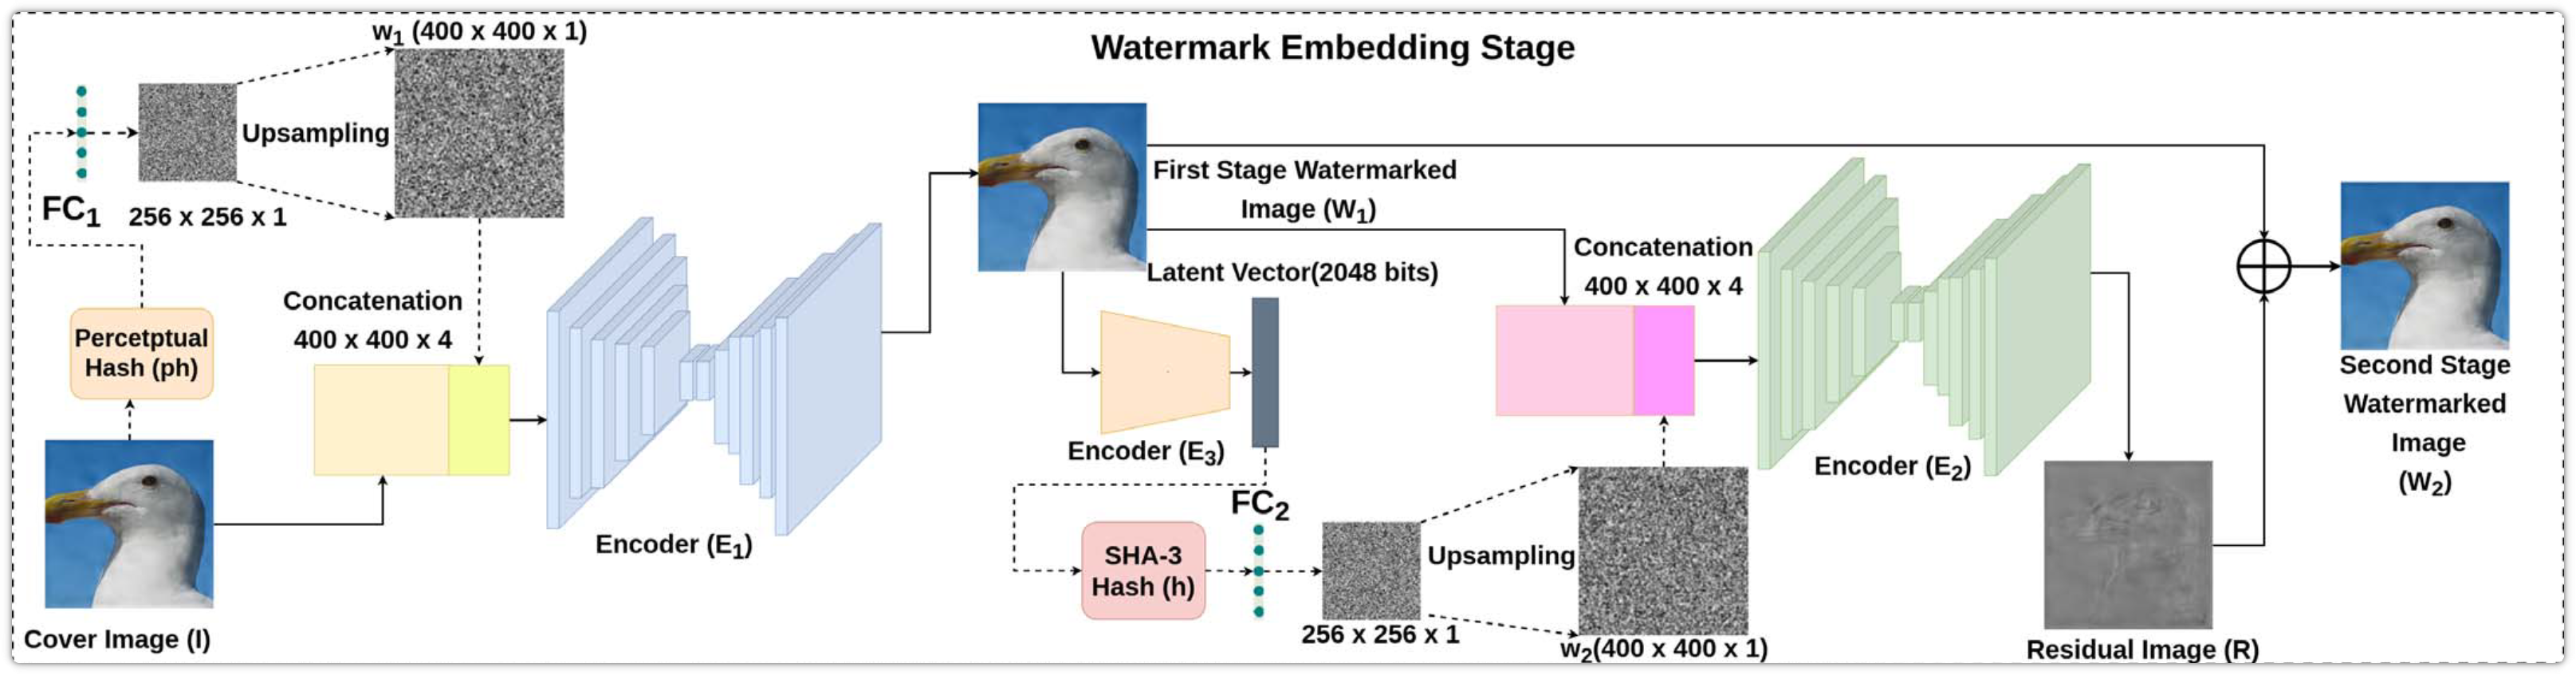
\includegraphics[width=\textwidth]{imgs/modelEmb.png}
  \caption{Watermark embedding process} %centre caption above image
  \label{fig:modelEmb}
  \Description{Watermark embedding process. The perceptual hash of the cover image is computed and passed through a pre-trained Fully Connected layer to produce a tensor, which is concatenated to the cover image and passed to the encoder network. The encoder network embeds the perceptual hash into the cover image and produces a watermarked image. The cryptographic hash of the watermarked image is computed and passed through the same pre-trained Fully Connected layer to produce another tensor, which is concatenated to the watermarked image and passed to the second encoder network. The second encoder network produces a residual image, which is added to the watermarked image to produce the final watermarked image.}
\end{figure}

The watermark embedding process is shown in the \autoref{fig:modelEmb}. The first step in our technique is to find the perceptual hash of the cover image $I$, which is our first watermark. There are different techniques for calculating the perceptual hash of an image.  We have chosen $DCT$-based perceptual hash as discussed in \autoref{subsubsec:perceptual-hash}. It has advantages in terms of robustness against distortions and attacks caused by content-preserving image manipulation. We compute $64$-bit $DCT$-based perceptual hash $ph$  of $I$, which is passed into a pre-trained Fully Connected layer ($FC$) to produce $256 \times 256 \times 1$  tensor and then upsampled to a $400 \times 400 \times 1$ tensor. The upsampled tensor is concatenated to $I$ as the fourth channel and passed to the encoder $E_1$. The job of $E_1$ is to embed $ph$  into $I$ as a watermark and produce a $400 \times 400 \times 3$ image as output, which is our first stage watermarked image $W_1$. It is ensured that $W_1$ will have the same perceptual hash as  $I$ by using three loss functions, which are residual regularization,  LPIPS perceptual loss, and critic loss. More details regarding these loss functions are discussed in Section-\ref{arch}.

Next, we compute the $256$-bit cryptographic hash $h$ of $W_1$ using $SHA$-$3$ and use it as our second watermark. The  $h$ is passed through the same pre-trained $FC$ to produce a $256 \times 256 \times 1$  tensor that is upsampled to  $400 \times 400 \times 1$ tensor. The upsampled tensor is concatenated to  $W_1$  as the fourth channel and  $400 \times 400 \times 4$ tensor is given as input to the second encoder $E_2$, which produces a residual image $R$ of resolution $400\times400\times3$ as the output.  The obtained $R$ is added to $W_1$, which yields the second stage watermarked image $W_2$ that is perceptually similar to the $I$. This addition of residual image ($R$)  does not change the perceptual hash and perceptual similarity of  $W_2$  with respect to $I$.  This is ensured by using appropriate loss functions while training. Adding to that,  we have also used two different techniques to embed the watermarks, thus reducing the chance of overlapping i.e, one watermark distorting the other. The technique followed for embedding $h$ into $W_1$ is inspired by the approach of Stegastamp~\cite{stegastamp}. Dual watermarking makes it convenient to perform different verification in one watermarked image. In our case, $W_2$ protects digital content copyright, content and source authentication.

\subsection{Watermark Extraction} \label{subsec:watermark-extraction}

\begin{figure}
  \centering
  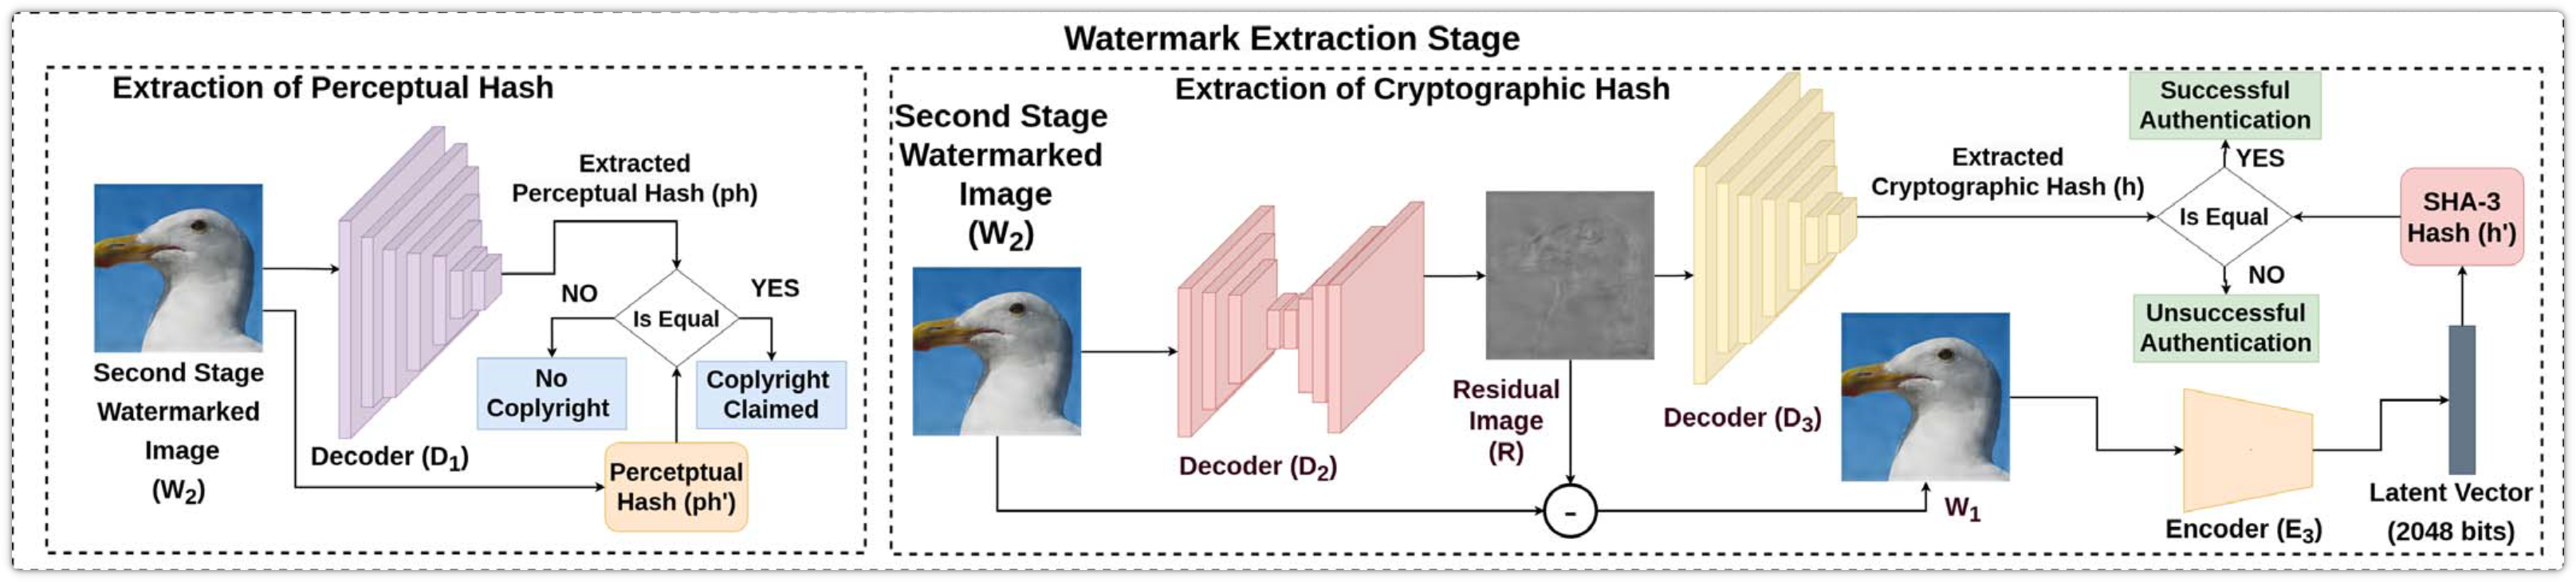
\includegraphics[width=\textwidth]{imgs/modelExt.png}
  \caption{Watermark extraction and verification process} %centre caption above image
  \label{fig:modelExt}
  \Description{Watermark extraction and verification process. The perceptual hash of the watermarked image is computed and compared with the extracted perceptual hash to verify ownership. The residual image is reconstructed from the watermarked image, and the cryptographic hash is extracted from the residual image. The cryptographic hash is compared with the computed cryptographic hash to verify content and source authenticity.}
\end{figure}

The watermark extraction and verification process is shown in \autoref{fig:modelExt}, which consists of two independent extraction phases:
\begin{enumerate}
  \item {\em Extraction phase $1$} is used for digital content ownership verification. We compute the perceptual hash ($h^\prime$) of $W_2$ using DCT transformation. Then $D_1$ extracts the embedded perceptual hash ($h$) from $W_2$. If the extracted and the computed perceptual hashes of  $W_2$ match, {\em i.e.,} $ph={ph}^\prime$, the image ownership is claimed.
  \item {\em Extraction phase $2$} is used for content and source authentication for the given dual watermarked image $W_2$. It uses two decoders: $D_2$ and $D_3$.  $D_2$  reconstructs a residual image ($R^{\prime}$) from given $W_2$.   $R^{\prime}$ is passed into $D_3$, which decodes the cryptographic hash ($h$) present in $R^{\prime}$. Subsequently, $R^{\prime}$ is subtracted from $W_2$, and the $SHA$-$3$ hash value ($h^\prime$) of the result is computed. If the cryptographic hash ($h$) extracted by  $D_3$ matches with the computed cryptographic hash ($h^\prime$), {\em i.e.,} $h={h}^\prime$, the authenticity of the content and source of the image is verified.
\end{enumerate}

A robust copyright protection mechanism should be able to extract the watermark successfully from the watermarked image and claim ownership even if the watermarked image is tampered with. Hence, $D_1$ used in the {\em Extraction phase $1$} should successfully extract the watermark from the tampered image to protect digital content copyright. To achieve this,  we have used a DCT-based perceptual hash, which is robust against distortions, compression, white Gaussian noises, and Gaussian blurring. To verify the authenticity of the content and source for an image, the hash of the image should not change. Therefore $D_2$ and $D_3$ are used in the {\em Extraction phase $2$}. It is ensured that  $D_2$ fails to reconstruct the residual image if the image is tampered with. Thus both $D_2$ and $D_3$ are trained on the images without adding any distortions.

\subsection{Network Architecture} \label{arch}

Our model consists of five networks ($E_1$, $E_2$, $D_1$, $D_2$ and $D_3$), which are trained in an end-to-end manner. We employ the U-Net~\cite{unet} architecture for both $E_1$ and $E_2$ with skip connections between the encoder and decoder layers of each U-net. It helps $E_1$ and $E_2$ to generate watermarked images that are perceptually similar to the input cover image.  Furthermore, the skip connections also preserve crucial spatial data and aid in recovering minute features that would have been lost during the downsampling of the image by the U-net encoders.

While embedding the perceptual hash, the emphasis is on the perceptual similarity between the reconstructed and original cover image, such that the perceptual hash does not change. In the same line, the hash is embedded and the residual image $R$ is generated by $E_2$, which is added to $W_1$ to produce $W_2$.

We employ a spatial transformer~\cite{spatial} to extract the perceptual hash, which takes $W_2$ as an input and extracts its embedded perceptual hash $ph$.   The spatial transformer used in $D_1$ provides invariance against various image transformations such as translation, scaling, rotation, cropping, deformations, change in brightness and contrast, etc. Decoding the cryptographic hash involves reconstructing $R^{\prime}$ using decoder $D_2$ and extracting $h$ from $R^{\prime}$ using $D_3$. U-Net is used to reconstruct $R^{\prime}$ using $D_2$,  whereas we use a simple convolution neural network with five convolution layers followed by two fully connected layers for extracting the hash from $R^{\prime}$ using $D_3$.

\subsection{Loss Function and Scheme Objective} \label{subsec:loss-function-and-scheme-objective}

For each loss function below, in order to decrease the difference caused by different order of two comparable images, we use the mean value of each loss function with two directions. For example, for $L_{PIPS}$, we compute the perceptual similarity between $I$ and $W_1$ as well as between $W_1$ and $I$, and then take the mean value of the two. The same applies to all other loss functions.

As mentioned earlier, the model is trained in an end-to-end manner.
Generally, embedding watermarks distorts the image, however, in our case, the perceptual hash and cryptographic hash introduce a small distortion in the cover image ($I$) such that the perceptual hash remains the same. Embedding the first watermark requires $I$ and the perceptual hash ($ph$) of $I$, which outputs $W_1$. To ensure minimal distortion while embedding $ph$ in $I$ as a watermark,  we used $L_2$ residual regularization ($L_{MSE}$), the LPIPS perceptual loss ($L_{PIPS}$) and a critic loss ($L_C$) functions. $L_{MSE}$ reduces the chance of the encoder to overfit while $L_{PIPS}$ and $L_C$ increases the perceptual similarity between $I$ and $W_1$.
$L_{PIPS}$ help us to compute the perceptual similarity between the two images corresponding to a predefined network. We use VGG-$19$ in our case~\cite{lpips} as the predefined network.
For given two images $A$ and $B$, the $L_{PIPS}$ corresponding to the $VGG$-$19$ is computed as follows:

\begin{equation}\label{eq:lpips}
  L_{PIPS} = \sum_{k} \tau^k (VGG^k (A) - VGG^k (B))
\end{equation}

In \autoref{eq:lpips}, features are extracted from $k$ layers of the $VGG$-$19$ network. The function  $\tau$ transforms deep embedding to a scalar LPIPS score. The final score between two images ($A$ and $B$) is computed and averaged for $k$ layers. {\em $L_C$} is calculated using a simple five-layer deep convolution neural network which classifies cover images and watermarked images using  Wasserstein loss~\cite{wass}.  It predicts whether a watermark is encoded in an image such that the embedding of the watermark can be improved.

\begin{equation}\label{eq:encoder1loss}
  L_{E_1} = \lambda_1 L_{MSE}(I, W_1) + \lambda_2 L_{PIPS}(W_1, I) + \lambda_3 L_C(I, W_1)
\end{equation}

\autoref{eq:encoder1loss} refers to the loss function used for $E_1$. Similarly, embedding the second watermark requires cryptographic hash ($h$) of $W_1$ and $W_1$, which outputs $W_2$. Thus we have used the same  $L_{MSE}$, $L_{PIPS}$, and $L_C$ loss for the encoder $E_2$ as referred in \autoref{eq:encoder2loss}.

\begin{equation}\label{eq:encoder2loss}
  L_{E_2} = \lambda_1 L_{MSE}(I, W_2) + \lambda_2 L_{PIPS}(W_2, I) + \lambda_3 L_C(I, W_2)
\end{equation}

$D_1$ uses binary cross-entropy loss to extract the embedded perceptual hash ($ph$) from $W_2$ (\autoref{eq:decoder1loss}). Decoder $D_2$ is used for reconstructing  $R^{\prime}$ from $W_2$ while decoder $D_3$ is used for extracting the embedded cryptographic hash ($h$) from $R^{\prime}$. After reconstructing  $R^{\prime}$ using $D_2$ it is compared with the original $R$ using $L_1$ loss, {$L_{PIPS}$} loss, and Mean Square Error ($L_{MSE}$) (\autoref{eq:decoder2loss}). Then $D_3$ is used to extract $h$ from $R^{\prime}$,  thus binary cross-entropy loss is used (\autoref{eq:decoder3loss}).

\begin{equation}\label{eq:decoder1loss}
  L_{D_1} = \lambda_7 L_{BCE}(D_1(W_2),ph)
\end{equation}

\begin{equation}\label{eq:decoder2loss}
  L_{D_2} = \lambda_4 L_1(R , R^{\prime}) +  \lambda_5 L_{PIPS}(R , R^{\prime}) + \lambda_ 6 L_{MSE}(R , R^{\prime})
\end{equation}

\begin{equation}\label{eq:decoder3loss}
  L_{D_3} = \lambda_d L_{BCE}(D_3(R^{\prime}),h)
\end{equation}

Training loss(\autoref{eq:total-loss}) is the sum of all five loss components ($L_{E_1},\: L_{E_2},\: L_{D_1},\: L_{D_2}, and \: L_{D_3}$), which is minimized and $\lambda$s are weight factors.

\begin{equation}\label{eq:total-loss}
  L= L_{E_1} + L_{E_2}+ L_{D_1} + L_{D_2} + L_{D_3}
\end{equation}

\subsection{Training of network}\label{subsec:training-of-network}

Our technique consists of two encoders and three decoders, which are trained together, as explained in \autoref{arch}. To ensure that the proposed technique works, we need to minimize the loss functions such that the model converges smoothly. The training procedure starts with embedding both the perceptual and cryptographic hash as watermarks into the cover image, as explained in \autoref{subsec:watermark-embedding}. This is followed by the extracting phase, as discussed in \autoref{subsec:watermark-extraction} for protecting digital content copyright as well as content and source authentication.

In order to protect digital content copyright, $D_1$ should extract the watermark even if $W_2$ is subject to content-preserving image manipulation such as JPEG compression, noise, blurring, cropping, deformations, etc. Hence, while training,  we performed random blurring, adding random noise, flipping, rotating, cropping, and compression to random watermarked images in the datasets such that $D_1$ can be robust in extracting the embedded perceptual hash. To reduce the impact of resizing and cropping on watermarked images,  we have restricted the embedding of perceptual hash in the centre portion of the images while training~\cite{stegastamp}. Decoders $D_2$ and $D_3$ are trained on the watermarked images without adding any distortions. This is due to the fact that minute changes in the watermarked image should be detected for successful content and source authentication.  We have trained three instances ({\em CelebA},  {\em Mirflickr} and combined $200$k images) of our model for $200$ epochs with a batch size of $32$. Early stopping and  $10$-fold cross-validation are employed to prevent the model from overfitting.  We have used Adam optimizer to optimize the parameters of all five sub-models in our technique. The learning rate is set as $1.0 \times 10^{-5}$, and we decay the learning rate by $0.2$ if the loss does not decrease within $10$ epochs.

\subsection{Android Application}\label{subsec:android-application}

We will implement an Android application to demonstrate the use of our model in a real-world application. The application will allow users to upload images, apply the watermarking technique, and verify ownership and authenticity. The app will be developed using Kotlin and the Android SDK, and it will provide a user-friendly interface for interacting with the watermarking model.

We have only implemented a simple Android application that allows users to upload images and apply the watermarking technique. The app will also provide options for verifying ownership for the owner. Which is to say that only the owner can verify the ownership of the image to check if the image belongs to him/her. The app will be developed using Kotlin and the Android SDK, and it will provide a user-friendly interface for interacting with the watermarking model.

Thanks to PyTorch Mobile, we can run the model on Android devices. The model will be converted to a format compatible with Android using the PyTorch Mobile library, which allows us to run PyTorch models on mobile devices.

\section{Tools and Technologies}\label{sec:tools-and-technologies}

% • List the tools, programming languages, and technologies you used for the project, explaining in particular detail any that were not considered in the proposal and/or interim report, or those you planned to use but did not.

% • Explain where and how you found or created the images used in the project. Specify any databases, websites, or sources that were used to gather images, and discuss the criteria for selecting or filtering images in the project. If any images or sets of images were initially planned to be used but turned out to be unsuitable or were replaced, explain why.

\subsection{Tools and Technologies}\label{subsec:tools-and-technologies}

The project will be implemented using the following tools and technologies:

\begin{itemize}
  \item \textbf{Programming Languages:} Python, Kotlin, Java
  \item \textbf{Libraries:} TensorFlow, OpenCV, NumPy, Matplotlib, PyTorch, Pillow, Android SDK
  \item \textbf{Frameworks:} TensorFlow, PyTorch
  \item \textbf{Tools:} NVIDIA GPUs CUDA SDK for training, Visual Studio Code for report writing, Git for version control, Android Studio for Android application development, Trello for task management, Discord for communication
\end{itemize}

\subsection{Dataset}\label{subsec:dataset}

We currently only used the Mirflickr dataset~\cite{mir} for training and testing the model. It consists of different types of images with varied contexts, lighting, and themes, perfect for exhibiting our techniques' generalization. The images are of resolution $500\times500$, which is downsampled to $400\times400$ for training.

To explore the generality of our technique, we used to want our evaluations on two datasets, CelebA~\cite{celeba} and Mirflickr~\cite{mir}. It is due to the time limitation that we only used the Mirflickr dataset for training and testing the model. The CelebA dataset is a large-scale face attribute dataset with more than 200,000 celebrity images, each with 40 attribute annotations. It contains a wide variety of facial images with different poses, expressions, and backgrounds, making it suitable for evaluating the robustness of our watermarking technique.

\section{Timeline}\label{sec:timeline}

% • Provide a timeline outlining major milestones and deadlines for your project. If parts of this timeline turned out significantly different from the timeline you’d originally proposed, explain why.

For now, we have the following milestones planned for the project:

\begin{itemize}
  \item \textbf{Milestone 1:} Finished early stage paper reading and collection (Completed: March 15, 2025)
  \item \textbf{Milestone 2:} Reached out to the author and got source code (Completed: March 25, 2025)
  \item \textbf{Milestone 3:} Implement the dual watermarking model and test(Incompleted)
  \item \textbf{Milestone 4:} Implement DeepRAFT and generate ideal pretrained model (Completed: April 15, 2025)
  \item \textbf{Milestone 5:} Implement the Android application (Completed: April 20, 2025)
  \item \textbf{Milestone 6:} Compare the performance of our model with existing techniques (Incompleted)
\end{itemize}

Compared to the original timeline, we have made multiple changes to the timeline.

Since on the early stage of the project, we have not fully thought about how the project will be implemented and what is exactly needed, we have thought everything linearly and we have not thought about the exact time for each step.
It was until we read the code and tried to reconstruct the model that we realized that this is not what we thought to be and far more complicated.
Since it is our first time fully implementing a neural network model processing images we have to spend a lot of time reading each function and compare them with different papers, codes and the original training process.
But we have learned a lot from this process and we are very happy that we have done it.
Even though we have not fully implemented the dual watermarking model, we have learned a lot on its structure and the way it works.
Since this summer is a long break, we decided to take further research on the dual watermarking model and try to implement it in the future.


\section{Outcomes}\label{sec:outcomes}

% • List specific objectives that you intended to achieve with your project, and what happened to them.

% • List any new applications you might have considered for your project as it developed.

We intented to achieve the following objectives with our project:

\begin{itemize}
  \item Develop a dual watermarking technique for image copyright protection and authentication.
  \item Implement an Android application to demonstrate the use of our model in a real-world application.
  \item Evaluate the performance of our model on different datasets and compare it with existing techniques.
\end{itemize}

However we have not yet completed the implementation of the dual watermarking technique, we have reached out to the original author of the paper and got their code.
But the code is not the same as the paper, and some of the crucial parts are not implemented yet.

But to make sure we can finish the project on time, we have implemented another model called DeepRAFT~(\url{https://github.com/xinghua-qu/DeepRAFT}) and forked the code from the original author.
After some modifications, we have successfully implemented the model and got the results and further implement the model into an Android application.

\subsection{Results}\label{subsec:results}

\subsubsection{Dual Watermarking}\label{subsubsec:dual-watermarking}

Here is some running results of our implementation of dual watermarking:

\begin{figure}[ht]
  \begin{minipage}{0.48\textwidth}
    \centering
    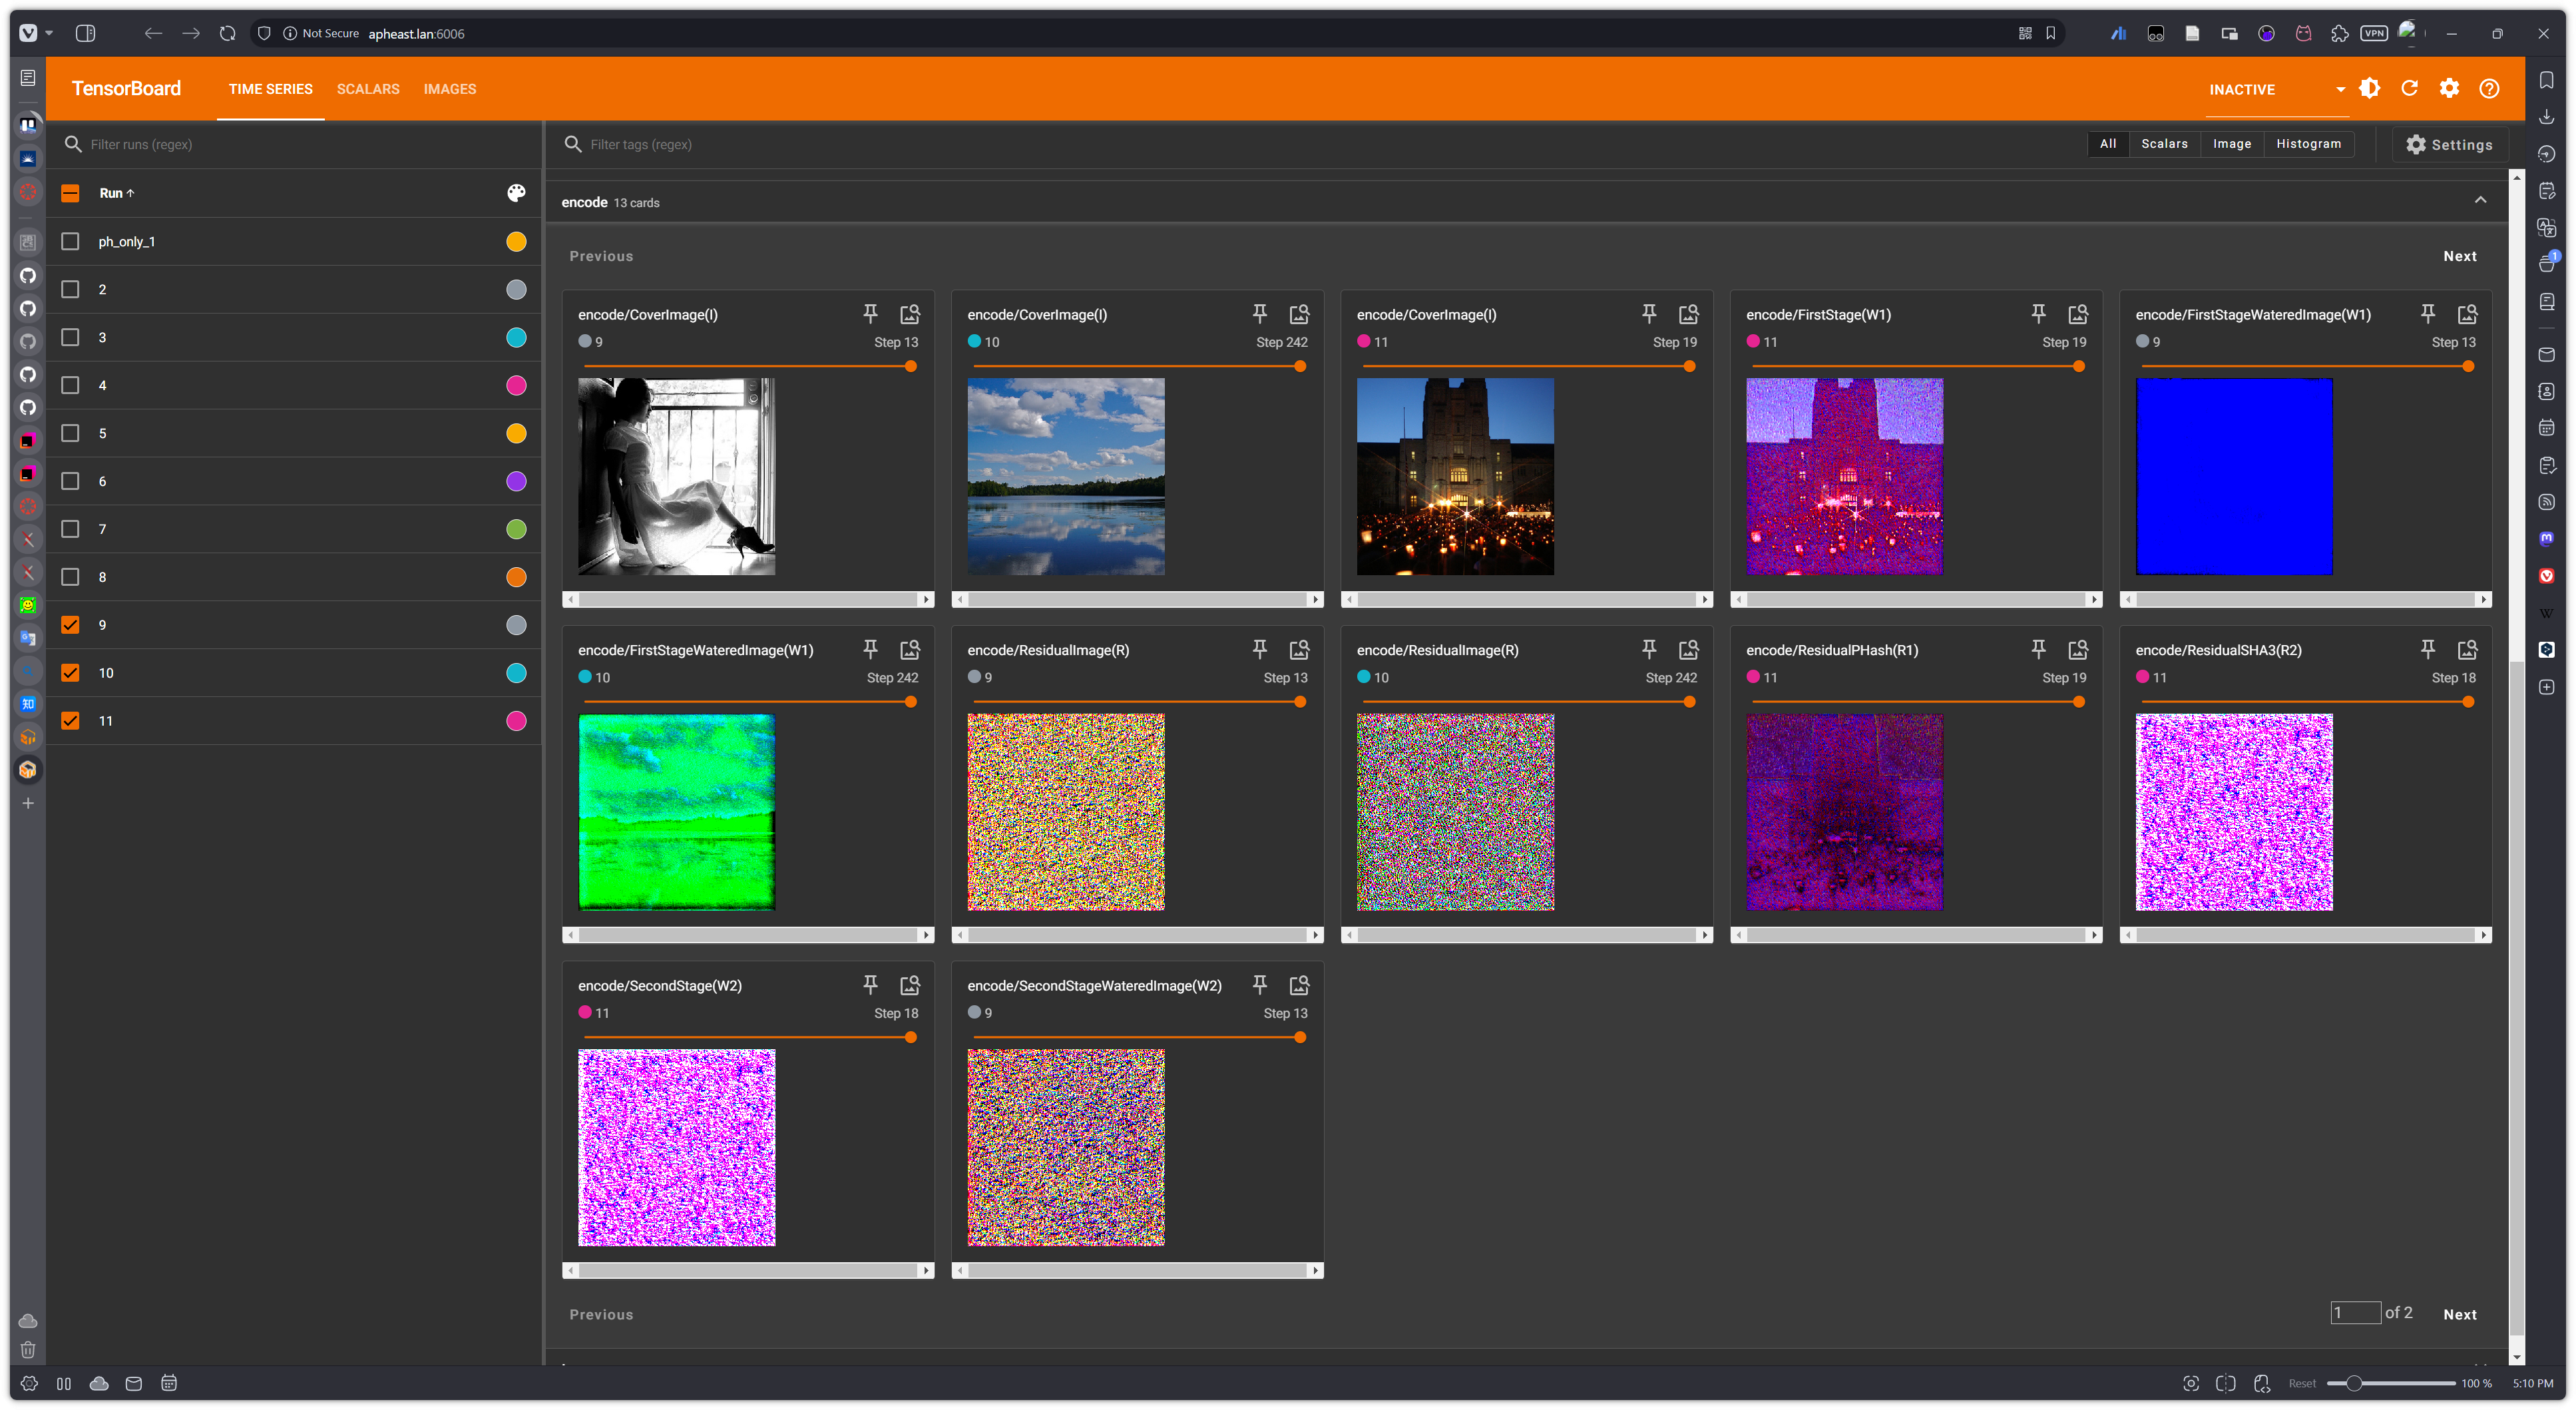
\includegraphics[width=\textwidth]{imgs/imageDual.png}
    \caption{Dual watermarking generated image}
    \label{fig:imageDual}
    \Description{Dual watermarking generated image. The image is generated by embedding the perceptual hash and cryptographic hash into the cover image using the dual watermarking technique. The image is perceptually similar to the original cover image.}
  \end{minipage}
  \hfill
  \begin{minipage}{0.48\textwidth}
    \centering
    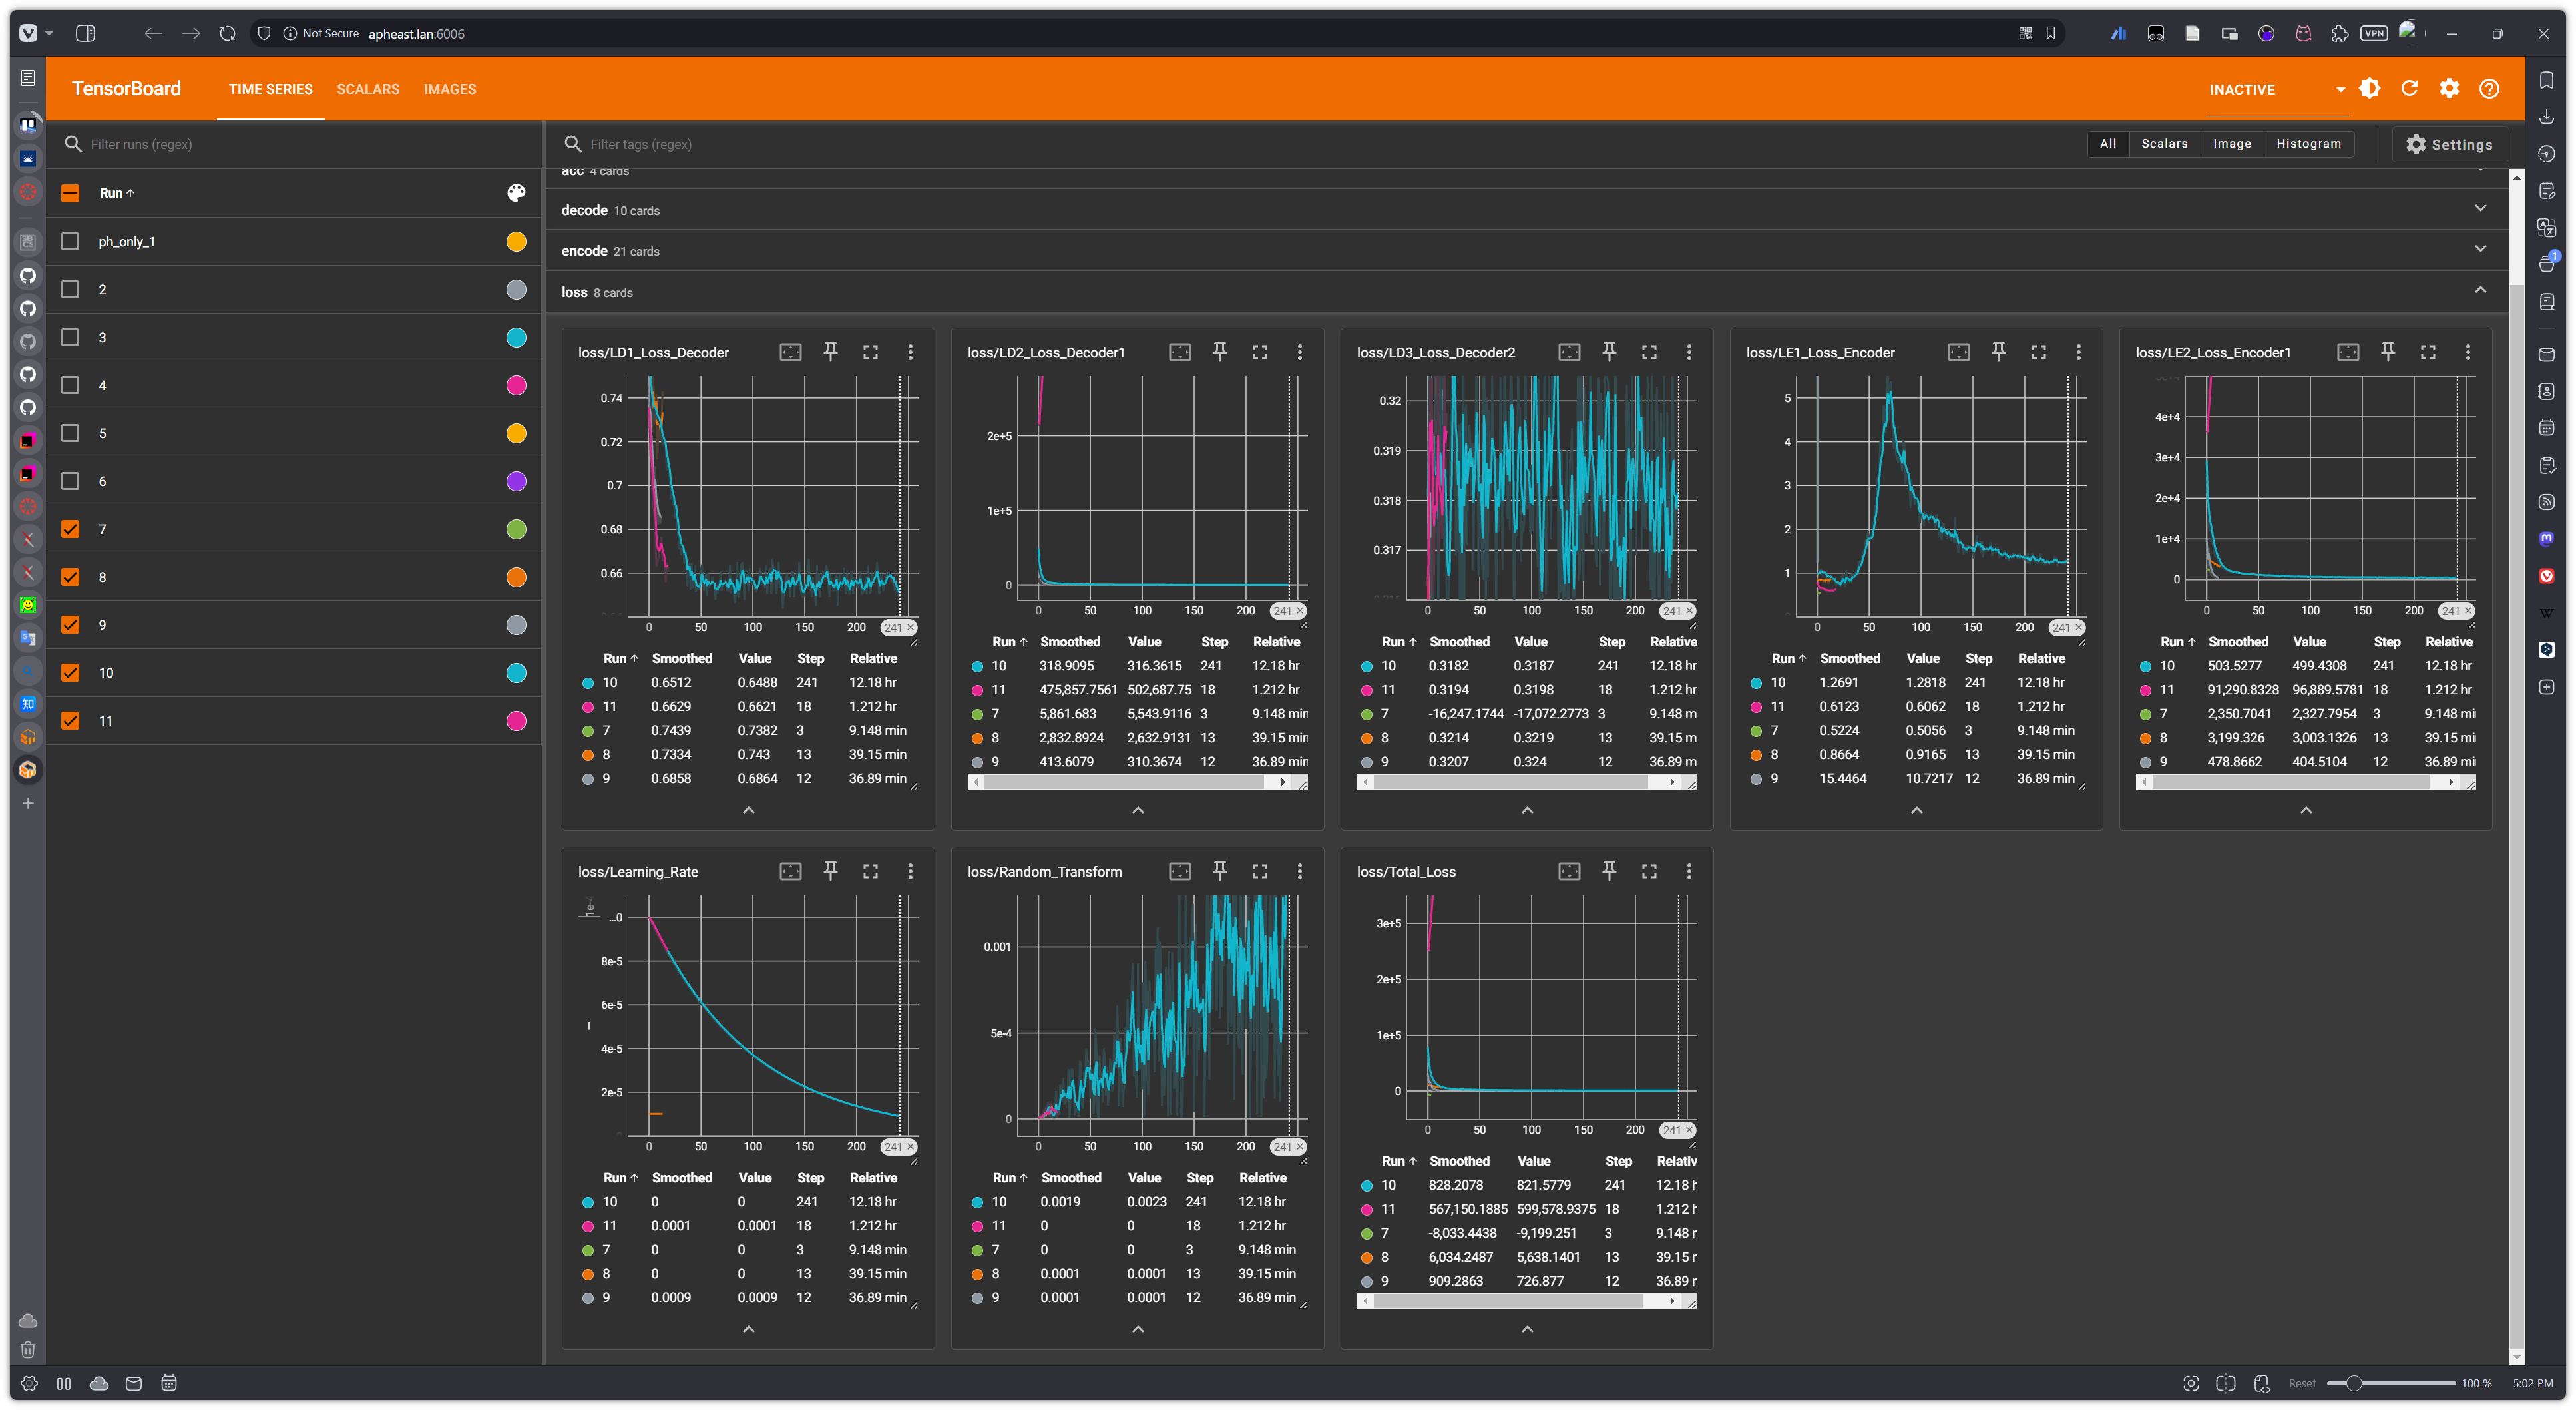
\includegraphics[width=\textwidth]{imgs/lossDual.png}
    \caption{Dual watermarking loss curve}
    \label{fig:lossDual}
    \Description{Dual watermarking loss curve. The loss curve shows the training loss of the dual watermarking model over time. The loss decreases over time, indicating that the model is learning.}
  \end{minipage}
\end{figure}

\subsubsection{DeepRAFT}\label{subsubsec:deepraft}

Here is some running results of our implementation of DeepRAFT:

\begin{figure}[ht]
  \begin{minipage}{0.31\textwidth}
    \centering
    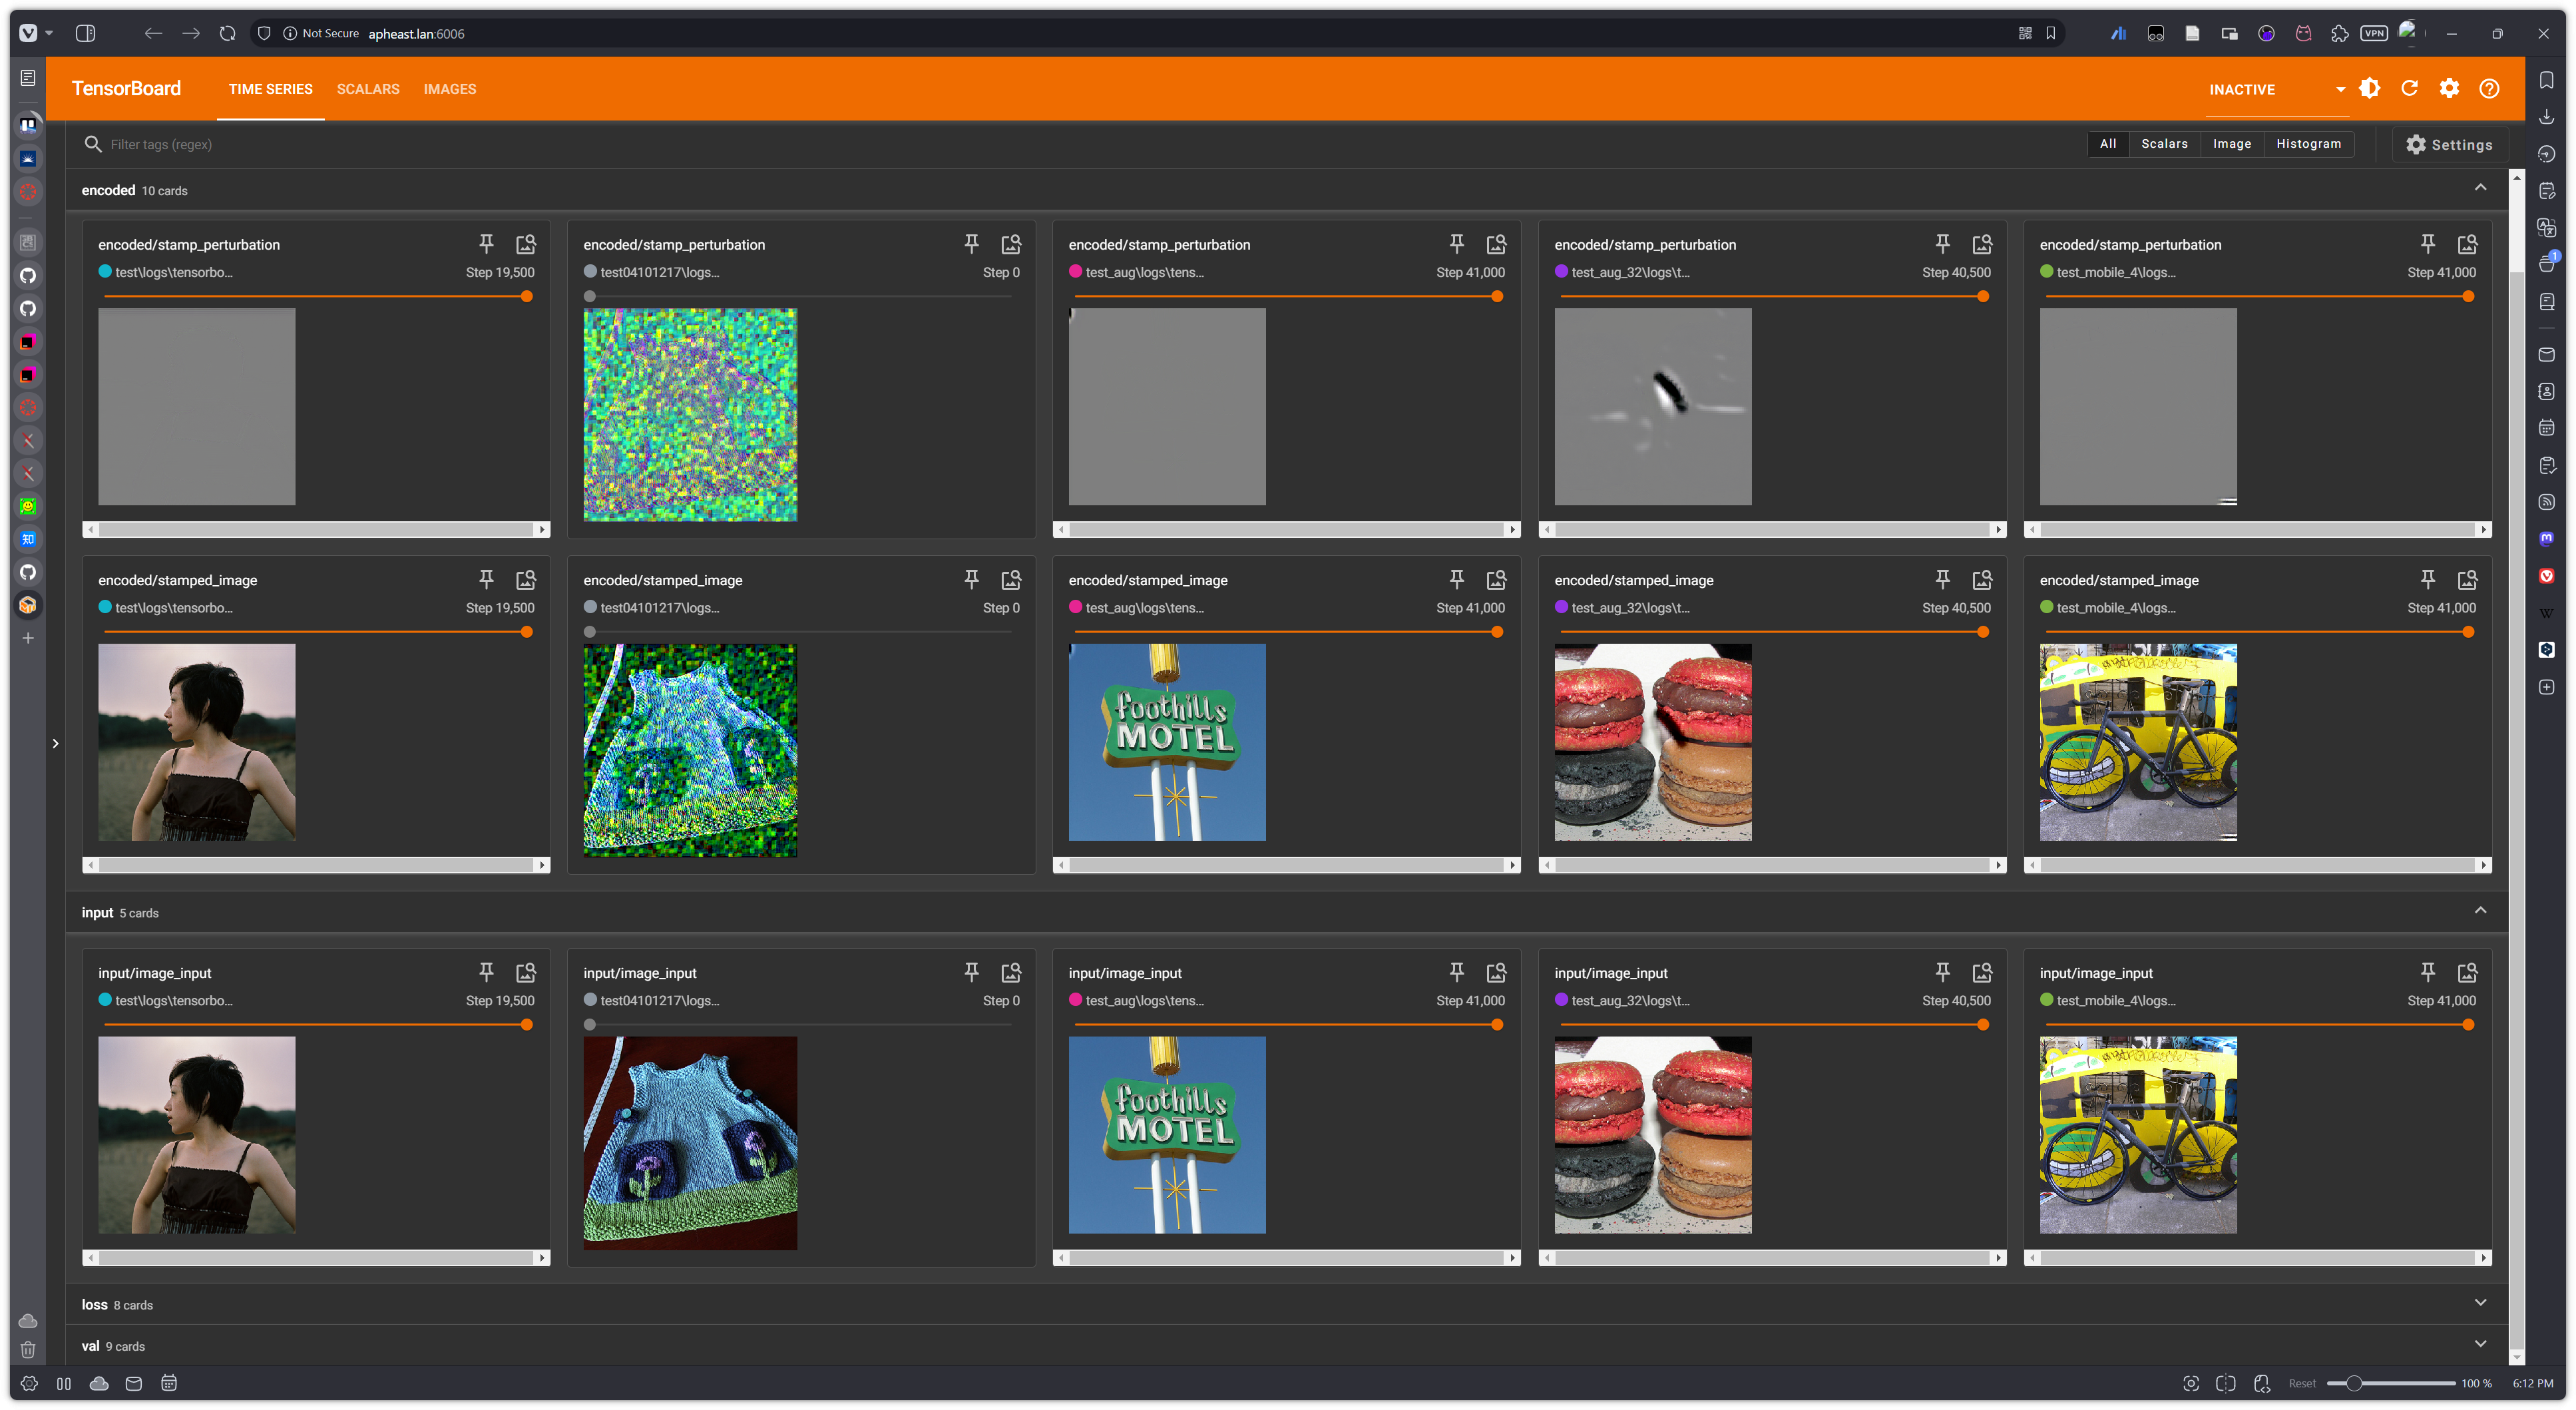
\includegraphics[width=\textwidth]{imgs/imageDeepRAFT.png}
    \caption{DeepRAFT image}
    \label{fig:imageDeepRAFT}
    \Description{DeepRAFT generated image. The image is generated by embedding the perceptual hash and cryptographic hash into the cover image using the DeepRAFT technique.}
  \end{minipage}
  \hfill
  \begin{minipage}{0.31\textwidth}
    \centering
    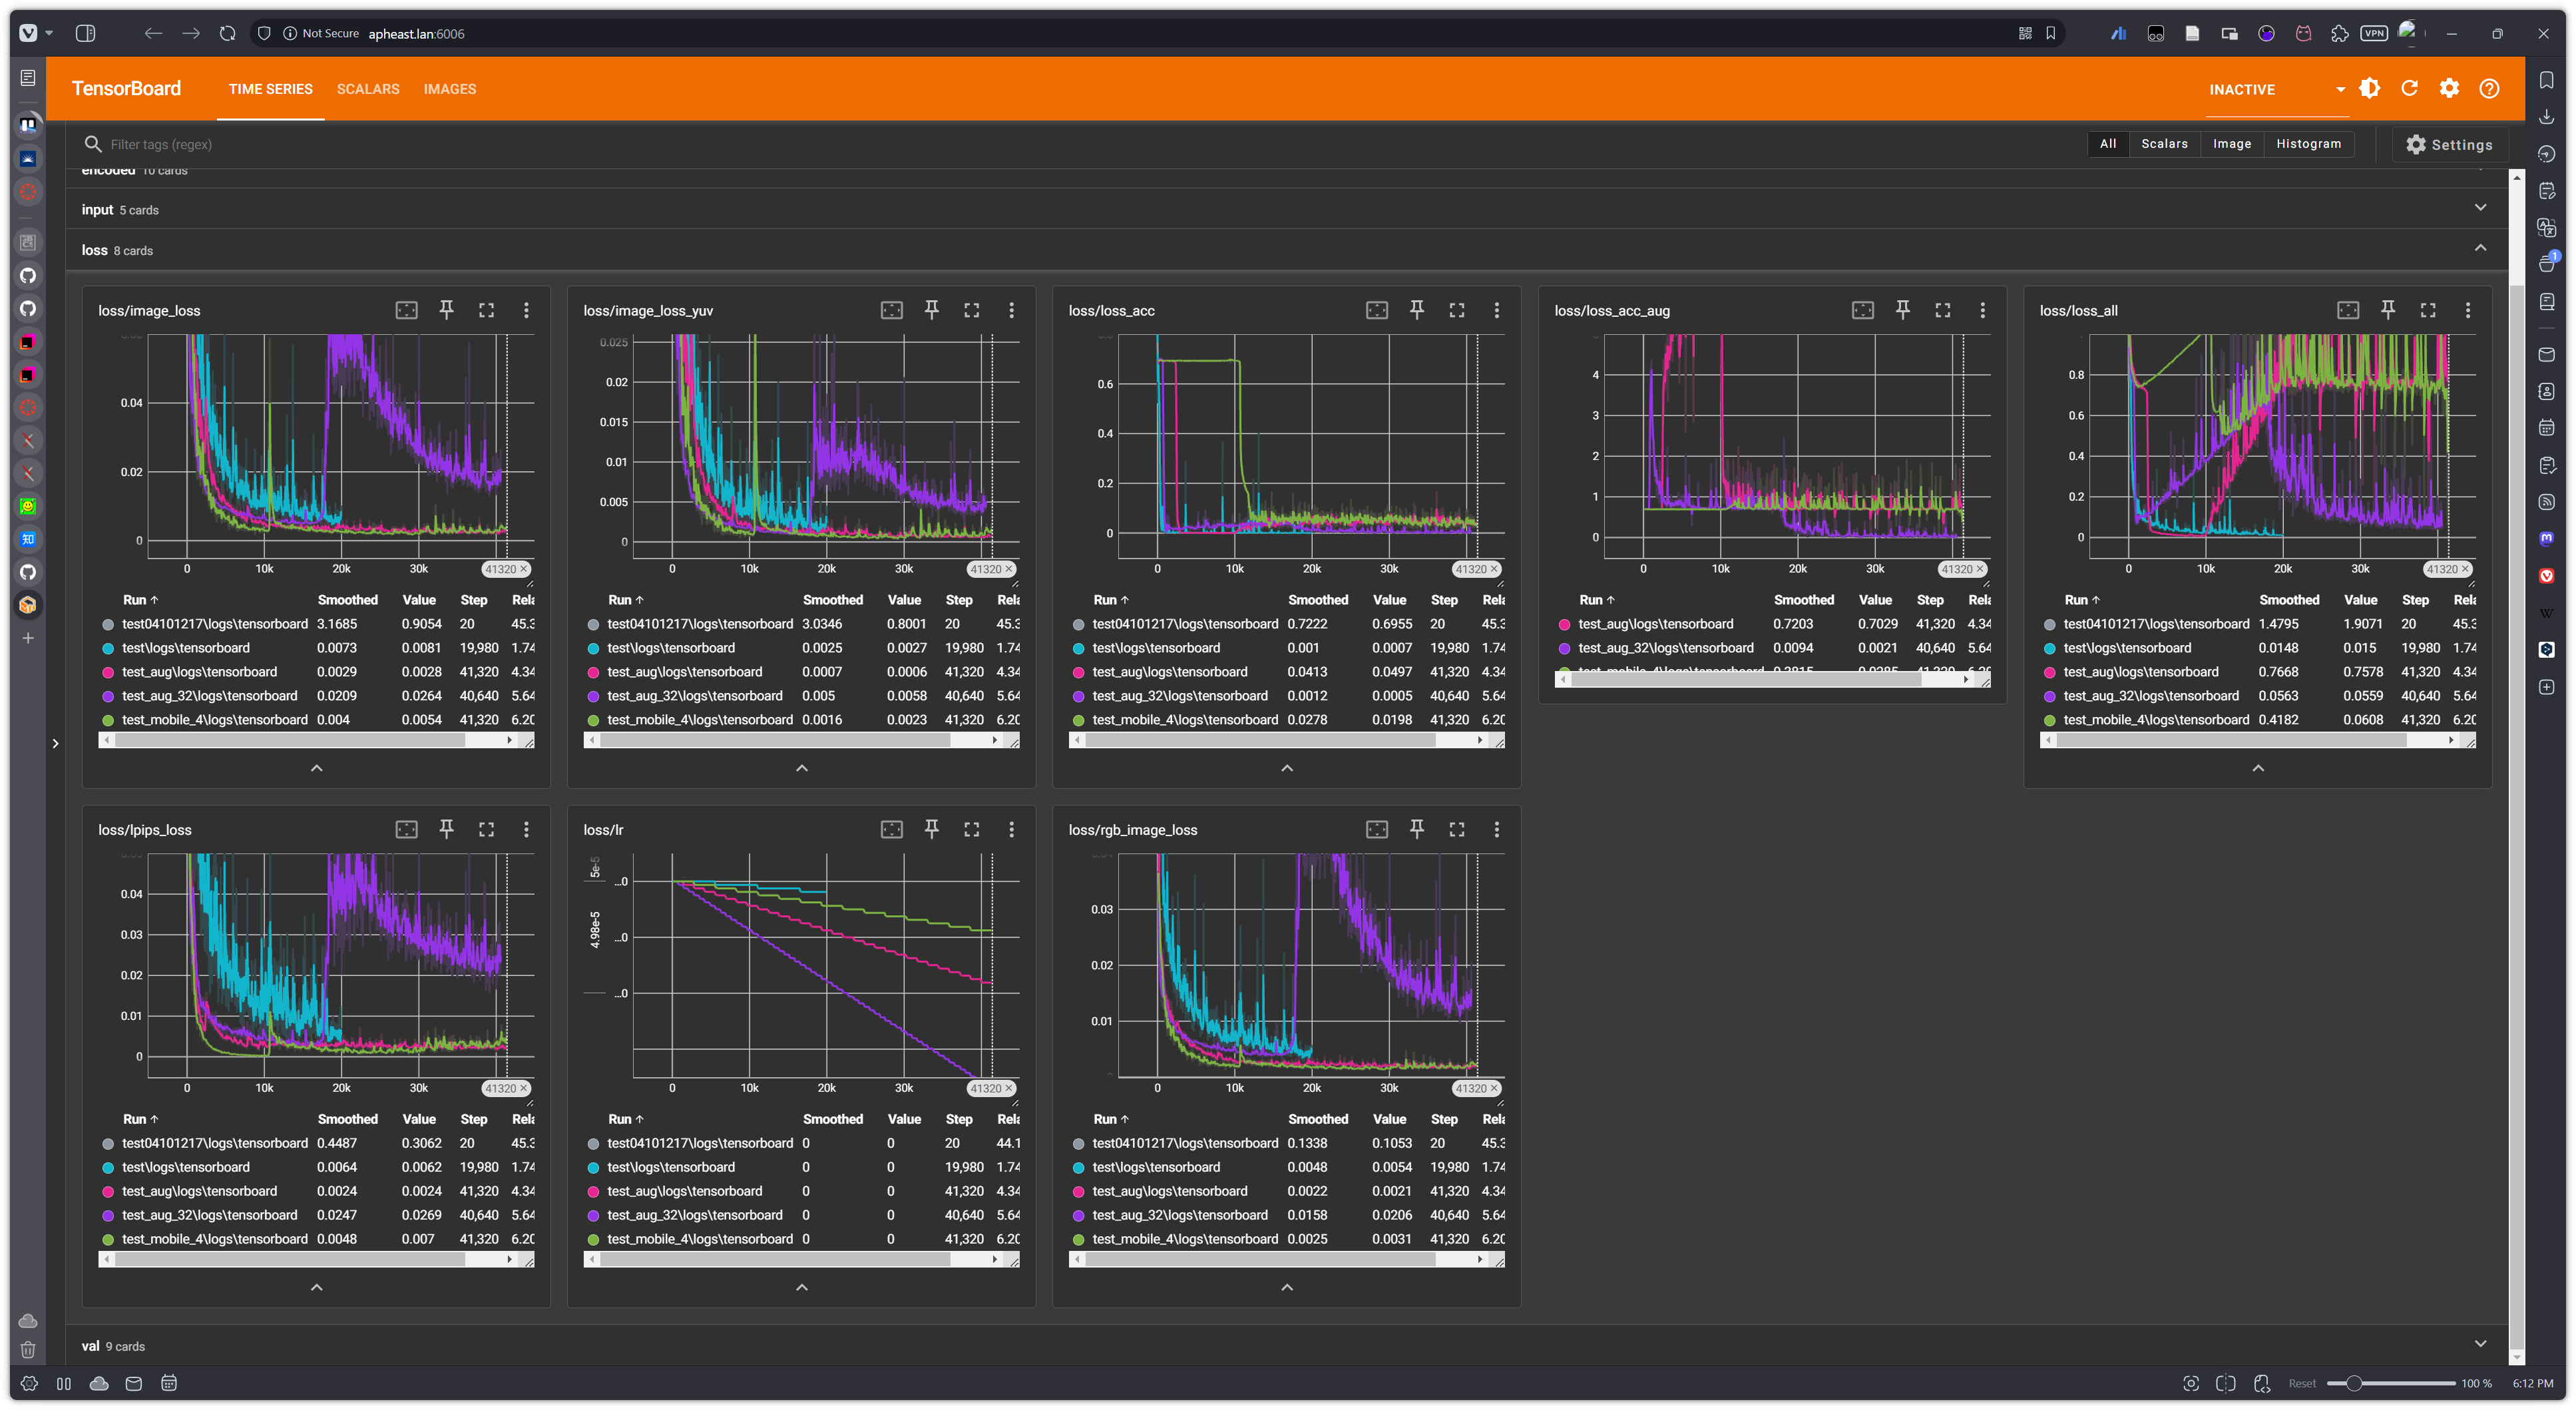
\includegraphics[width=\textwidth]{imgs/lossDeepRAFT.png}
    \caption{DeepRAFT loss curve}
    \label{fig:lossDeepRAFT}
    \Description{DeepRAFT loss curve. The loss curve shows the training loss of the DeepRAFT model over time.}
  \end{minipage}
  \hfill
  \begin{minipage}{0.31\textwidth}
    \centering
    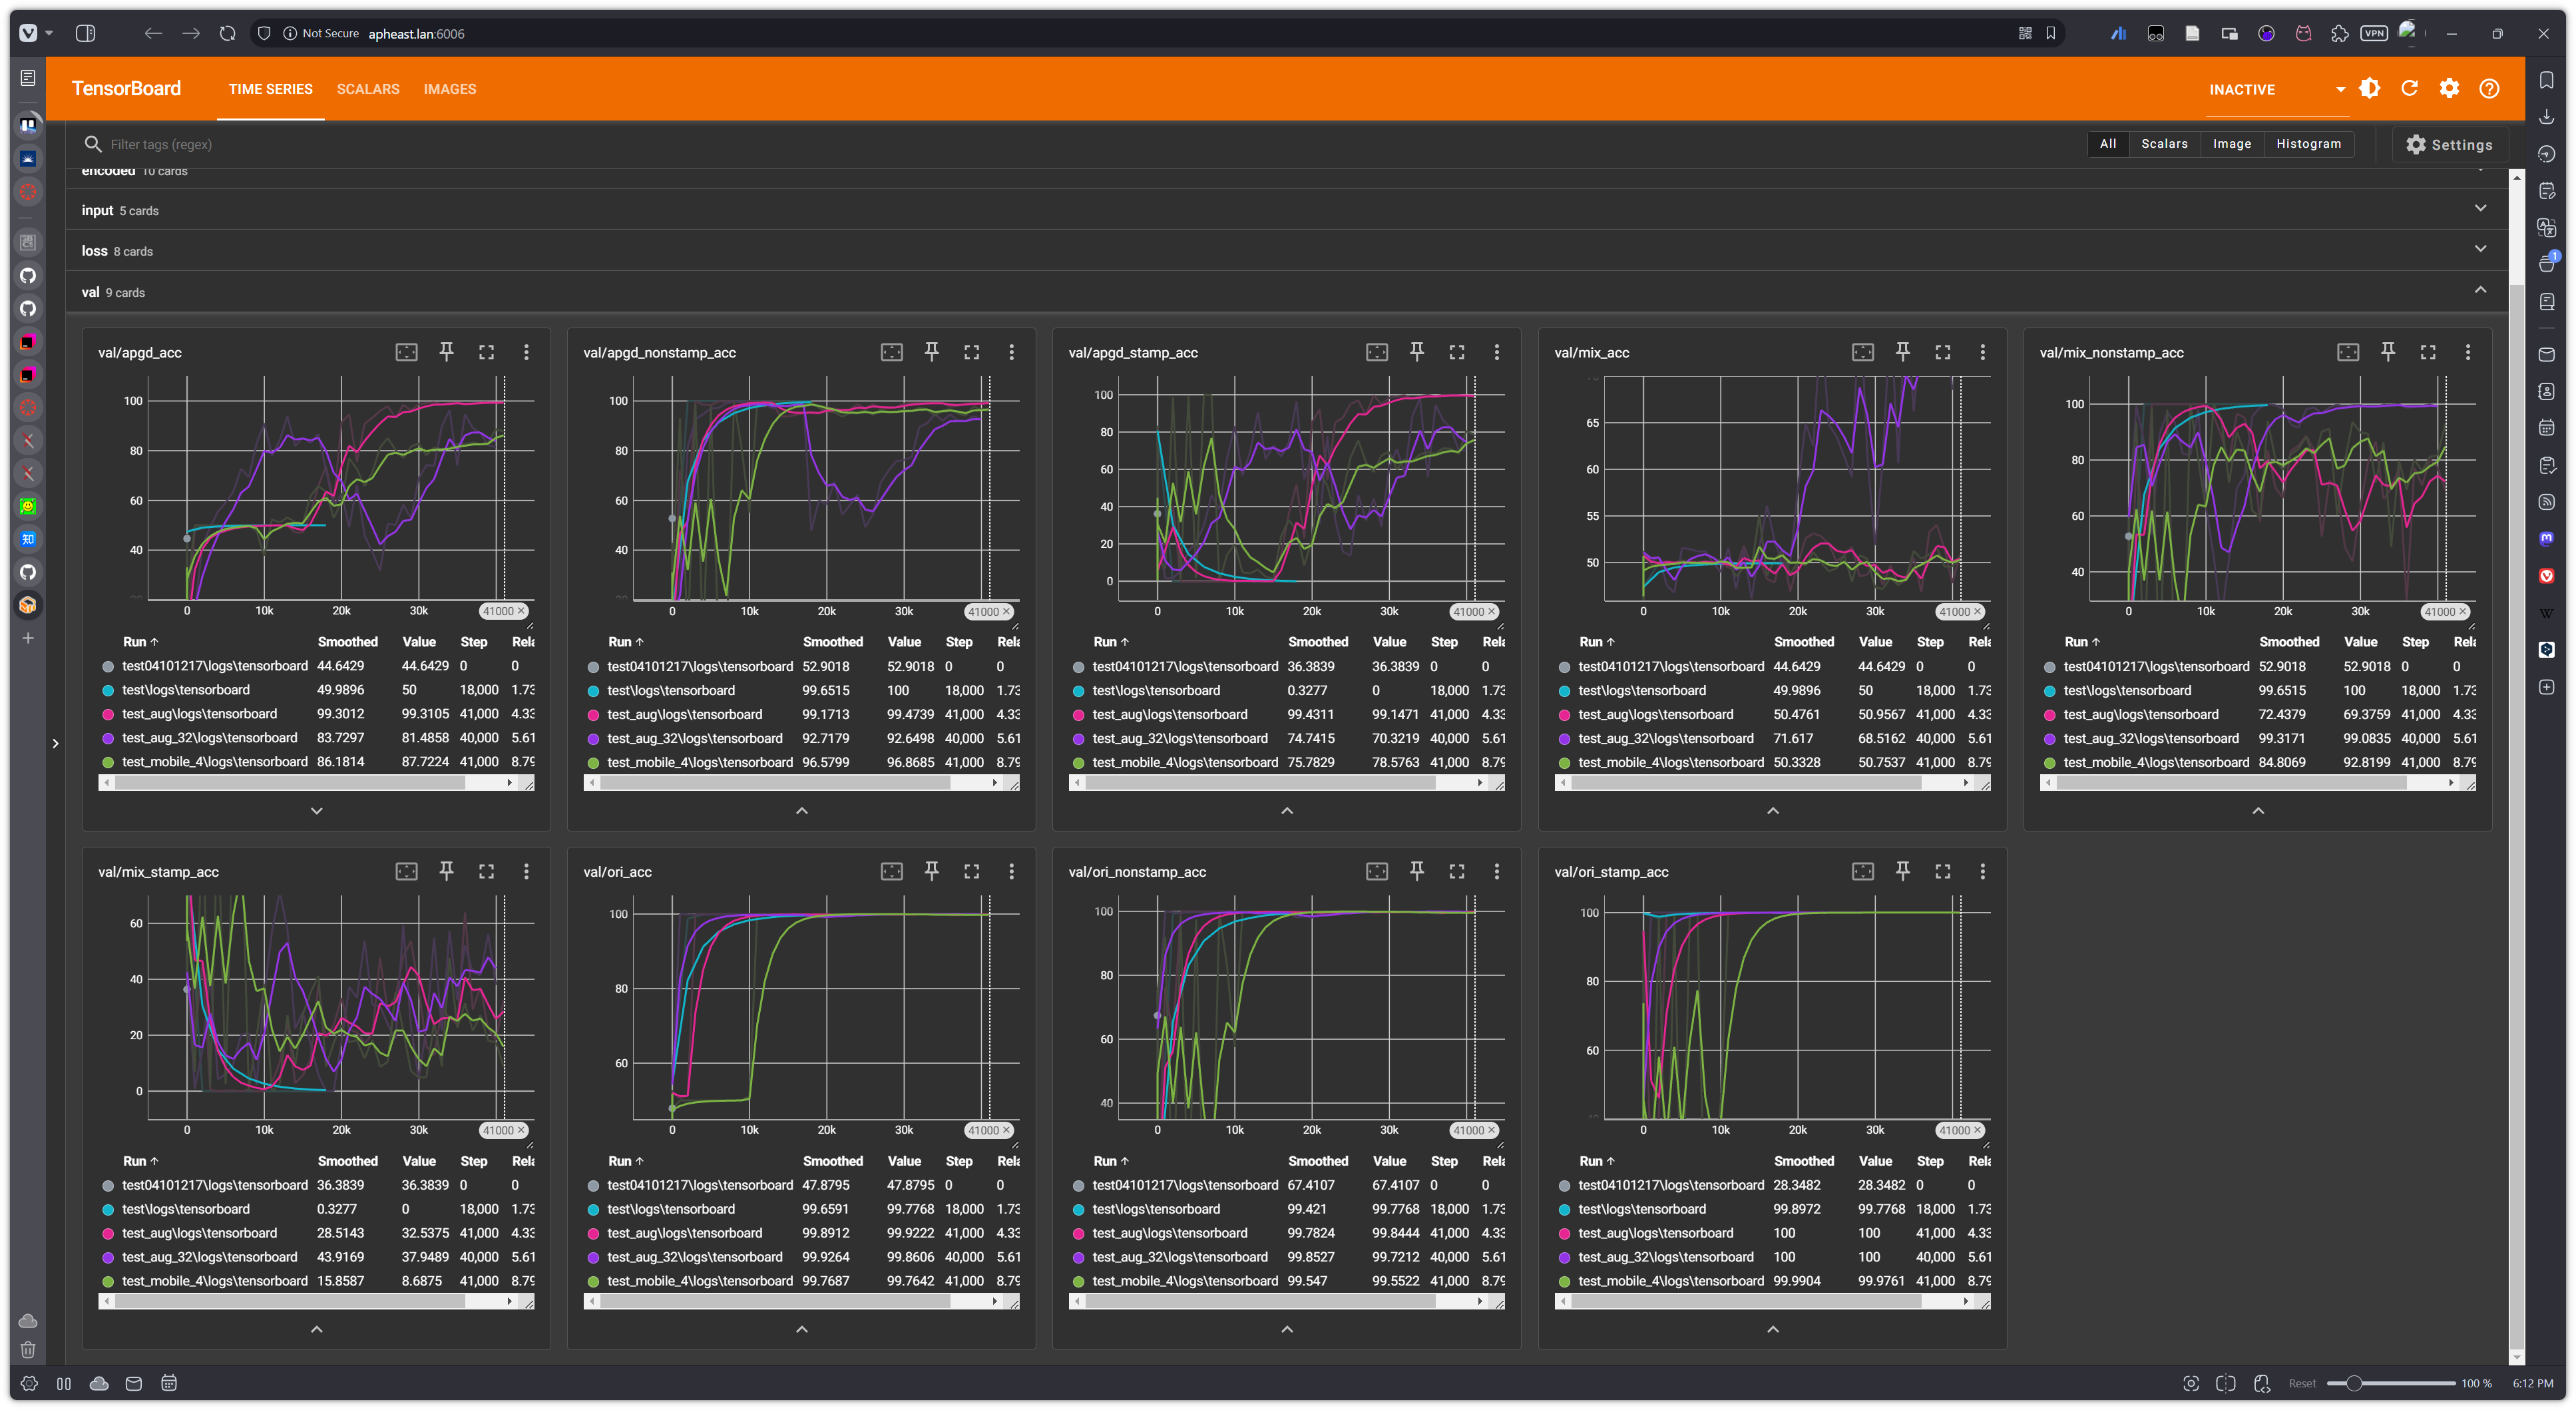
\includegraphics[width=\textwidth]{imgs/accDeepRAFT.png}
    \caption{DeepRAFT acc curve}
    \label{fig:accDeepRAFT}
    \Description{DeepRAFT accuracy curve. The accuracy curve shows the training accuracy of the DeepRAFT model over time.}
  \end{minipage}
\end{figure}

\subsubsection{Android Application}\label{subsubsec:android-application}

Here is some running screenshots of our implementation of Android application:

\begin{figure}[ht]
  \begin{minipage}{0.31\textwidth}
    \centering
    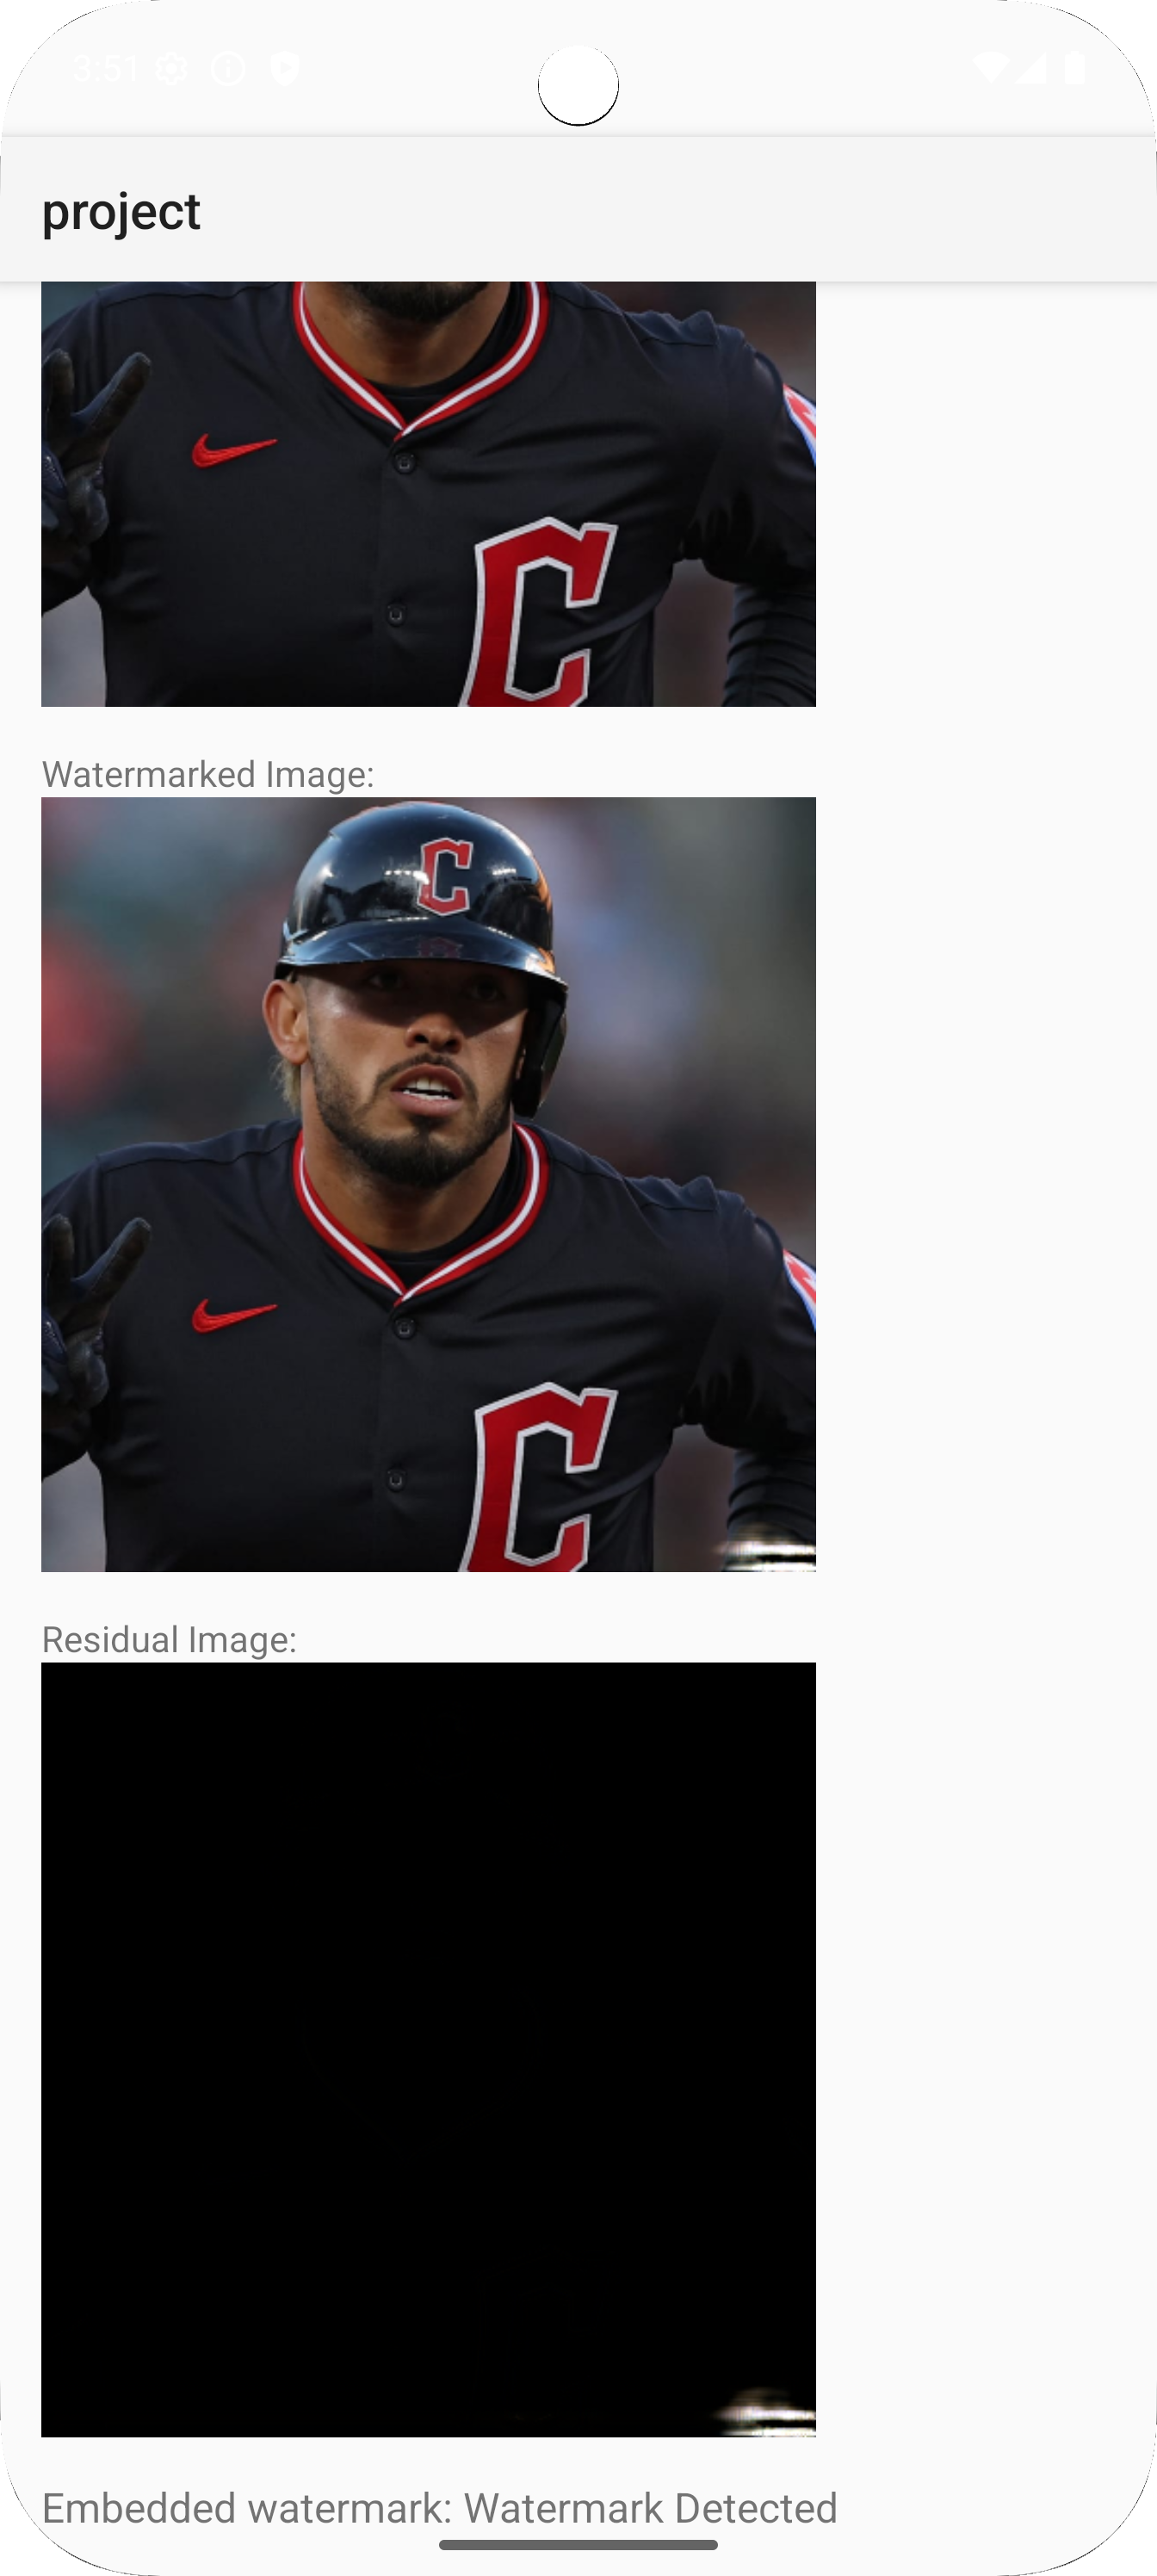
\includegraphics[width=\textwidth]{imgs/androidEnc.png}
    \caption{Watermark Embeded}
    \label{fig:androidEnc}
    \Description{Successful image encoding. The image is successfully encoded using the dual watermarking technique. The image is perceptually similar to the original cover image.}
  \end{minipage}
  \hfill
  \begin{minipage}{0.31\textwidth}
    \centering
    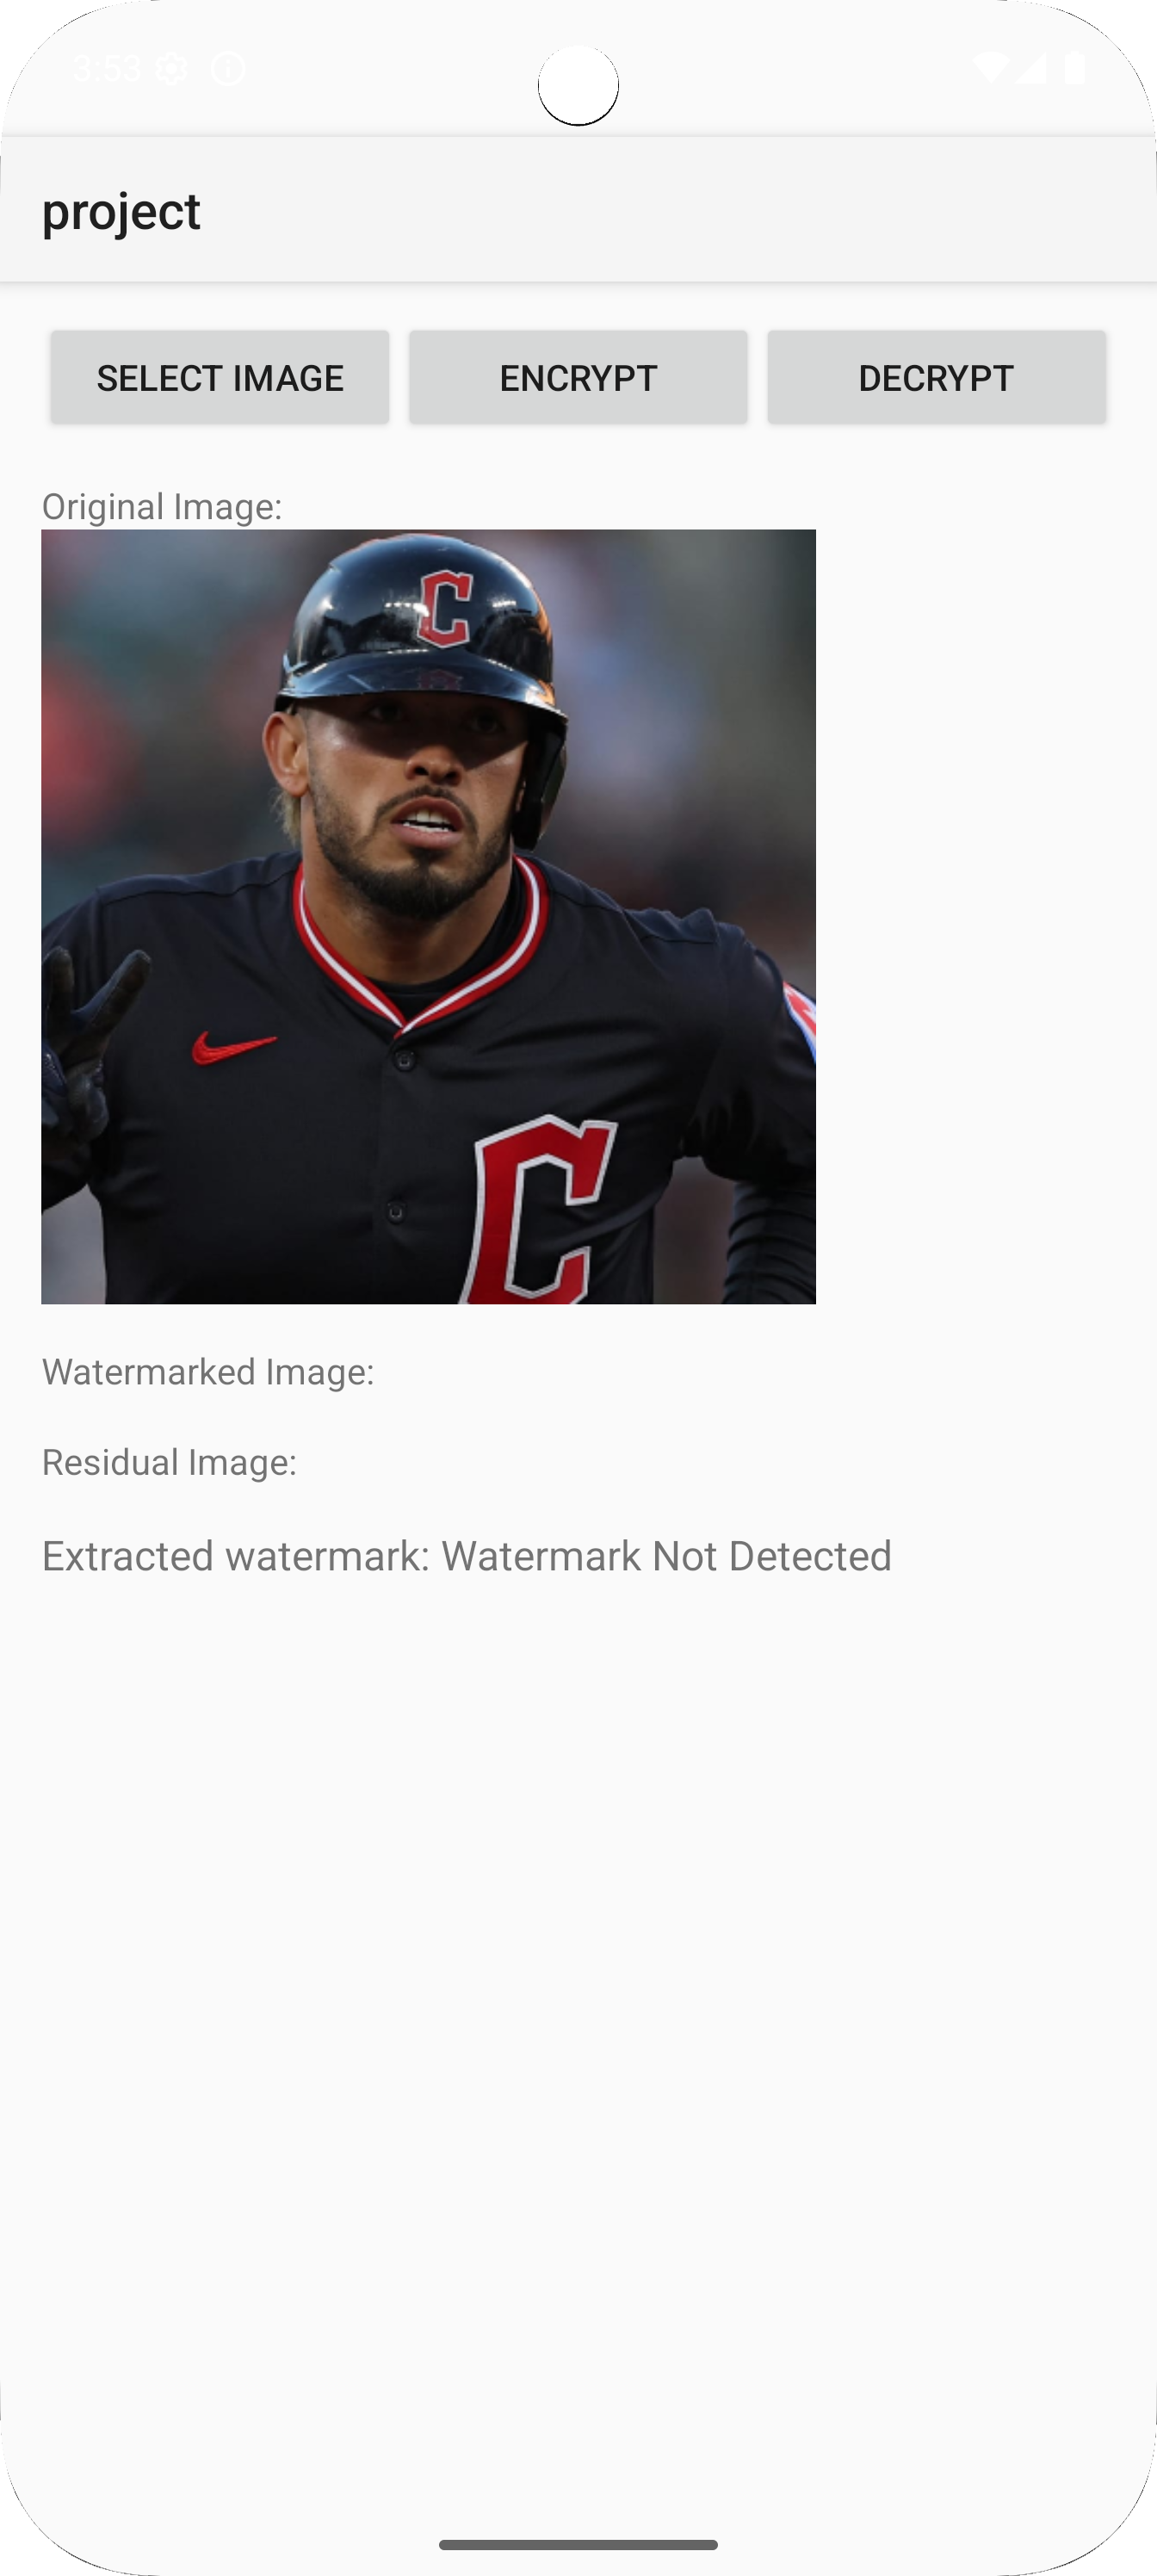
\includegraphics[width=\textwidth]{imgs/androidDecUndetected.png}
    \caption{No watermark detected}
    \label{fig:androidDecUndetected}
    \Description{No watermark detected. The image is not detected as a watermarked image. The image is not perceptually similar to the original cover image.}
  \end{minipage}
  \hfill
  \begin{minipage}{0.31\textwidth}
    \centering
    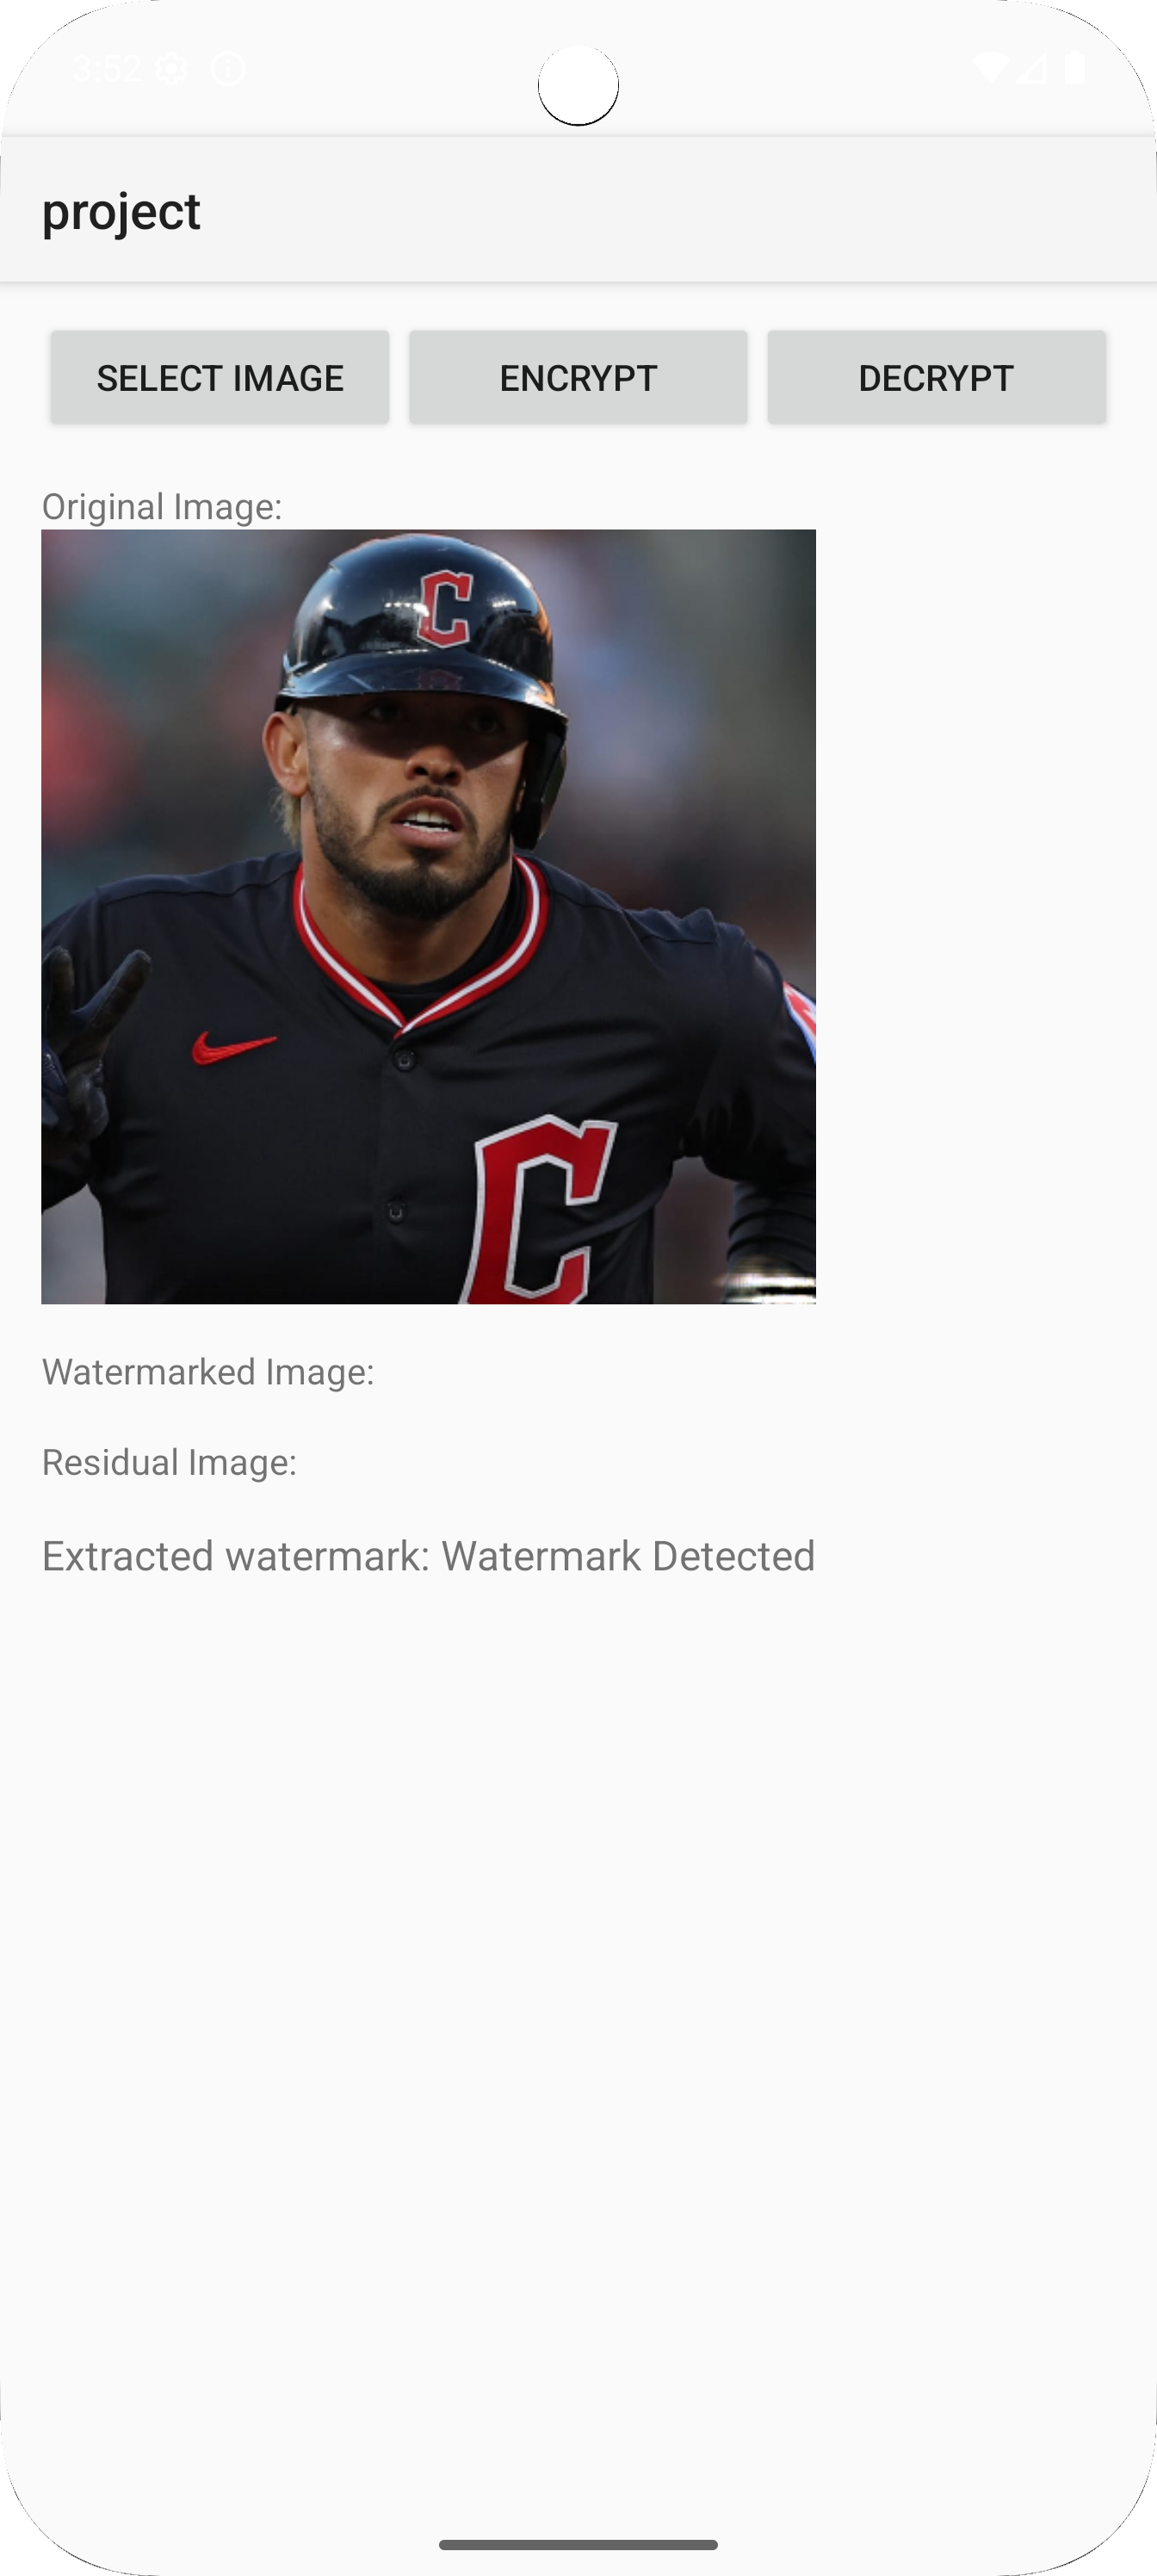
\includegraphics[width=\textwidth]{imgs/androidDecDetected.png}
    \caption{Watermark detected}
    \label{fig:androidDecDetected}
    \Description{Watermark detected. The image is detected as a watermarked image. The image is perceptually similar to the original cover image.}
  \end{minipage}
\end{figure}

\subsection{Code Repository}\label{subsec:code-repository}

The code for the project is hosted on GitHub at the following link:
\begin{itemize}
  \item {\em Dual Watermarking }\url{https://github.com/Aphcity/dual-channel-watermarking}
  \item {\em DeepRAFT Watermarking }\url{https://github.com/Aphcity/DeepRAFT}
  \item {\em Android Application }\url{https://github.com/YihaoCWRU/Watermark_Android}
\end{itemize}

\section{Further Work}\label{sec:further-work}

% • Briefly describe what you would do to continue the project if you had more time or resources to expand its scope.

% • Describe other work that could be based off of the project’s results.

Since we have not yet completed the implementation of the dual watermarking technique, but we have learned a lot from other models like DeepRAFT and Stegastamp, we will further implement the dual watermarking technique and compare the performance of our model with existing techniques.
To make the next coming steps more clear, we have listed the following steps:

\begin{itemize}
  \item Implement Encoder 2 and Decoder 2 for the dual watermarking model
  \item Implement the loss function and training the model for the dual watermarking model where we think the loss function of Encoder 1 and Encoder 2 should be further modified to make sure the watermarked image is perceptually similar to the original image.
  \item Train the auto encoder model to get the hash latent vector and then use the hash latent vector to generate the residual image.
  \item Further examine the whole watermarking process and make sure it is reasonable and robust.
  \item Try to further implement the Android application and make it more user-friendly and can use camera to scan multiple images lively.
  \item Compare the performance of our model with existing techniques and make sure it is robust and can be used in real-world applications.
\end{itemize}

\section{Work Division}\label{sec:work-division}

% • Briefly review how the team originally planned to distribute tasks and responsibilities among team members.

% • Describe any changes to the original plan, and what circumstances prompted those changes.

% • Discuss how collaboration and communication were managed within the team.

For specific tasks, we have finished following tasks:

For Chentao Fan:
\begin{itemize}
  \item Collected latest papers, codes and reading them
  \item Reached out to the original author and getting the source code
  \item Implemented Encoder 1 and Decoder 1
  \item Implemented Perceptual Hash and verify its correctness
  \item Implemented Loss function and training the model
  \item Implemented thorough logging system to record the training process using Tensorboard
  \item Compatible with PyTorch Mobile and convert the model to a format compatible with Android
\end{itemize}

For Yihao Zhang:
\begin{itemize}
  \item Prepared the dataset
  \item Implemented Stegastamp and generated ideal pretrained model(ABANDONED, not able to optimize for mobile since it is TensorFlow model)
  \item Implemented DeepRAFT and generated ideal pretrained model
  \item Implemented VINE and generated ideal pretrained model(ABANDONED, not able to get the code and optimize for mobile)
  \item Implemented the Android application
  \item Prepared the presentation
\end{itemize}

Compared to the original plan, we have made multiple changes to the work division.

we have originally planned to implement the dual watermarking model, a DCT based, and a DWT based model.
And do the comparison between the three models.
But due to the time limitation, we have only implemented the dual watermarking model and it is still not fully implemented yet.
So we have implemented another model called DeepRAFT~\cite{quOnlyYouDeep2022} and forked the code from the original author.
After some modifications, we have successfully implemented the model and got the results and further implement the model into an Android application.
Meanwhile, we have also tested some other models like Stegastamp and VINE, but since Stegastamp~\cite{tancikStegaStampInvisibleHyperlinks2020} is a TensorFlow model and not able to optimize for mobile, we have abandoned it.
As for VINE, even the model is published on Huggingface and according to the paper~\cite{luRobustWatermarkingUsing2025}, we are not able to get the code and optimize for mobile, so we have abandoned it as well.

\bibliographystyle{ACM-Reference-Format}
\bibliography{sample-base}

\end{document}
\endinput